% !TEX root = ../report.tex

\chapter{State Of The Art}
\minitoc
\label{chap:SotA}

This section will present and discuss previous work in the field of recommender
systems. First out is recommender system fundamentals which cover the main recommender
system techniques which the techniques described later in the chapter are based.
Next up is a round up of some existing solutions to the cold start problem, followed
by fashion recommender systems, session based approaches and lastly a summary
of how recommender systems can be evaluated.

\clearpage

% !TEX root = ../../report.tex

\section{Recommender Systems foundations}
\label{sec:recsys}
Recommender systems have become an important research topic since the
introduction of Tapestry \cite{Goldberg1992}, the first collaborative filtering
system back in 1992. Recommender systems now play an important role in many of
the most popular web-sites such as Amazon, YouTube, Netflix, TripAdvisor,
Last.fm, and IMDb. In its most common formulation the recommendation problem is
reduced to the problem of estimating the preference/rating of items that have
not been seen by a user. Usually, this estimation is based on one or more of
the following assumptions:

\begin{itemize}
\item You are like your friends
\item You are like people who do similar things that you do
\item You like things that are similar to things you already like
\item You are influenced by experts and the opinions of others.
\end{itemize}

Once we have estimated these ratings we can recommend the items with the
highest rating to the user. These recommendations relate to various
decision-making processes, such as what items to buy, what music to listen to,
or what online news to read. Recommender systems are usually classified into
the following categories, based on how the recommendations are made
\cite{Adomavicius2005}.

\begin{itemize}
\item \emph{Content-based recommendations:} The user will be recommended items with similar content to the ones the user preferred in the past;
\item \emph{Collaborative recommendations:} The user will be recommended items that people with similar testes and preferences have liked in the past;
\item \emph{Hybrid approaches:} These methods combine collaborative and content-based methods.
\end{itemize}

\subsection{Content Based Filtering}

In a content-based system, we must construct a user \emph{profile}
$ContentBasedProfile(c)$ or each user $c$, which is a record or collection of
the attributes which characterizes each item $Content(s)$ of all the items
$s_{i} \epsilon S$ previously rated by user $c$. For example in a fashion
recommender system the content-based recommender system tries to understand the
commonalities among the items user $c$ has rated highly in the past (color,
brand, store, price, etc.). Then recommend items that have a high degree of
similarity to these items. $ContentBasedProfile(c)$ can be designed as a vector
of weights $(w_{c1} ... w_{ck})$, where each weight $w_{ci}$ denotes the
importance of the keyword $k_{i}$ to user $c$.

Items that can be recommended to the user can often be stored in a database
table. Figure \ref{figure:contentbaseddb} shows a simple database with rows
describing 5 items that have been rated by 3 users. The column names starting
with $X_{n}$ are the properties of the items, often referred to as
"attributes".

\begin{figure}[H]
    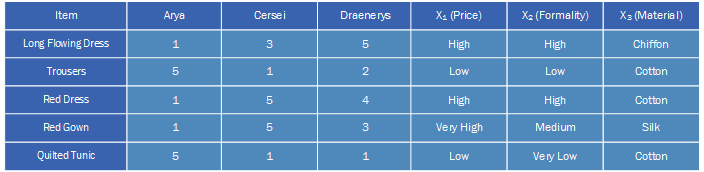
\includegraphics[width=5in]{image/contentbaseddb.png}
    \centering
    \caption[A clothing database]{A clothing database. Rows are items, columns are users and item attributes}
    \label{figure:contentbaseddb}
\end{figure}

From the rating matrix and content properties one can then construct a
$ContentBasedProfile(c)$ for each user $c$, for the user Arya one could imagine
it would look something like this.

\begin{figure}[H]
    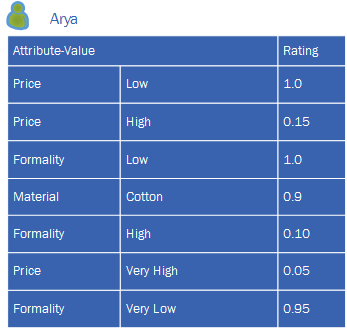
\includegraphics[width=2in]{image/contentprofile.png}
    \centering
    \caption[Content Profile Example]{Content Profile Example}
    \label{figure:contentprofile}
\end{figure}

The recommendation process consists of matching up the attributes of the user
profile against the attributes of an item. The result is a relevance judgment
that represents the user's level of interest in that object. The utility $u(c,
s)$ of item $s$ for user $c$ is estimated based on the utilities $u(c, s_{i})$
assigned by user c to items $s_{i} \epsilon S$ that exhibit a similarity to
item $s$. E.g. for the user Arya items with the attributes low price and low
formality could safely be recommended as they fit her user profile, and have
similar characteristics to the items which she previously have rated highly.
The utility function $r(u, i)$ is usually defined as:

\begin{equation}
r(u,i) = score(ContentBasedProfile(u), Content(i)).
\end{equation}

\subsection{Collaborative Filtering}
\label{subsec:cf}

The goal of collaborative filtering methods is to suggest new items or to
predict the utility $u(c, s)$ of a certain item s for a particular user c based
on the user's previous activities and/or likings and similarity to other users.
In a typical CF scenario, there is a list of $n$ users $C = {c_{1}, ... c_{n}}$
and a list of $m$ items $S = {s_{1},...s_{m}}$. Each user $c_{i}$ has a list of
items $S_{si}$, which the user have expressed her opinion about, which makes up
our rating matrix of size $S \times C$. More formally, the utility $u(c, s)$ of
item $s$ for user $c$ is estimated based on the utilities $u(c_{j}, s)$
assigned to item $s$ by the users $c_{j} \epsilon C$, which can be considered
"similar" to the active user $c$. This is exemplified in Figure
\ref{figure:ratingmatrix}. For example, in our fashion recommender system, in
order to recommend clothes to user $c$, the collaborative filtering method must
find the "peers" of users $c$, which share the same tastes in clothes (user
which tend to enjoy similar clothes). Then, recommend the clothes that are most
liked among these "peers".

\begin{figure}[H]
    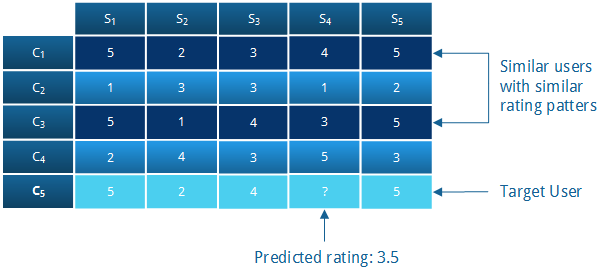
\includegraphics[width=5in]{image/ratingmatrix.png}
    \centering
    \caption[Collaborative filtering rating matrix]{Collaborative filtering rating matrix}
    \label{figure:ratingmatrix}
\end{figure}

Researchers have devised a number of collaborative filtering algorithms that
can be divided into two main categories: Memory-based and Model-based
algorithms \cite{Su2009}.\linebreak[4]

\begin{figure}[H]
    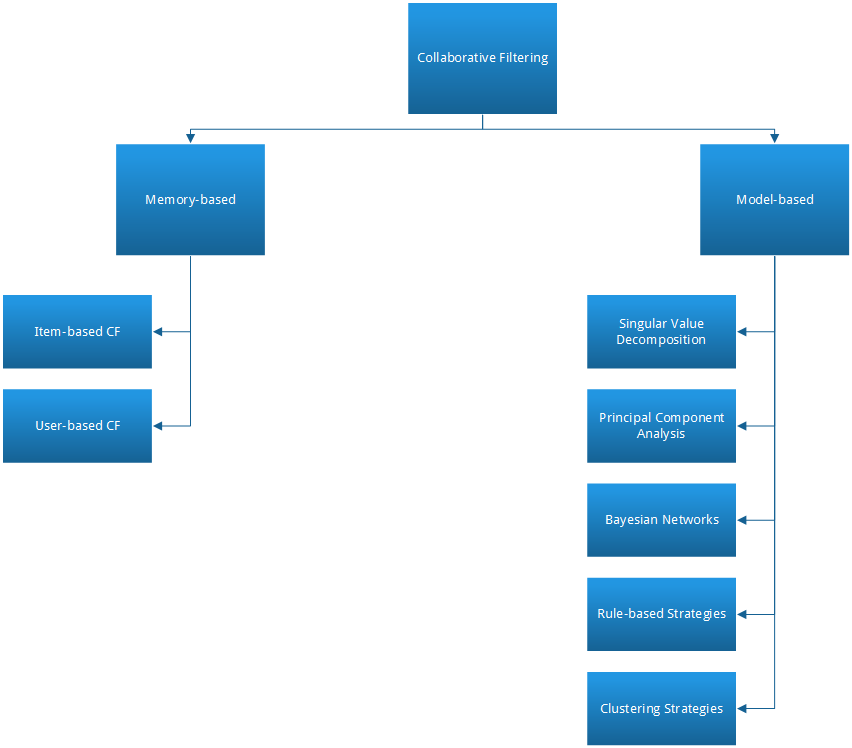
\includegraphics[width=5in]{image/cftaxonomy.png}
    \centering
    \caption[Classification of collaborative filtering techniques]{Classification of collaborative filtering techniques}
    \label{figure:cftaxonomy}
\end{figure}

\subsubsection{Memory-based Methods}

Memory-based Collaborative Filtering methods utilize the entire user-item
database to generate predictions. More formally, the value of an unknown
utility $u(c,s)$ for user $c$ and item $s$ is usually computed by taking the
weighted average of the utilities assigned by the $N$ most similar users for
the same item $s$. The similarity between user $c$ and $c'$, $sim(c, c')$ is
used as the weight. The more similar a user $c'$ is to $c$, the more weight is
given to the utility $u(c', s)$, and thus, will carry more weight in the
prediction for $u(c,s)$.

\begin{equation}
\label{equation:cfratingprediction}
u(c,s) = k * \sum_{c' \epsilon C} sim(c, c') * u(c',s)
\end{equation}

Where k serves as a normalization factor, usually being $1/|C|$. Various
approaches have been used to compute the similarity $sim(c, c')$ between the
users. Generally these approaches are based on the rating similarities for
items both users have rated. The most popular similarity measure is The Pearson
Correlation Coefficient. Equation \ref{equation:pearson} shows how to calculate
the Pearson Correlation Coefficient between two users $c$ and $c'$, Here
$S_{cc'}$ is the set of items both users have in \emph{common}.

\begin{equation}
sim(c, c') = \frac{\sum_{s \epsilon S_{cc'}} (u(c, s)-\bar{u_{c}})(u(c',s)-\bar{u_{c'}})}{\sqrt[•]{\sum_{s \epsilon S_{cc'}} (u(c, s)-\bar{u_{c}})^{2}(u(c',s)-\bar{u_{c'}})^{2}}}
\label{equation:pearson}
\end{equation}

Where $u_{c}$ is the mean utility of user $c$. The Pearson Correlation
Coefficient and other similarity measures such as consine based approaches are
more commonly known user-based collaborative filtering.\newline

Item-based Top-N Recommendation methods calculates the similarity between items
instead of users. In these approaches, the historical information is analyzed
to identify the relations between items such that a purchase of another item
(or set of items) often leads to the purchase of another item. These models are
often used since they quickly can recommend a set of items, and have shown to
produce recommendation results comparable or better than traditional user-based
approaches \cite{Karypis2001}.

The algorithm first computes the $k$ most similar items for each item according
to the ratings given by users they both share. Once the most similar items are
found, the prediction is then computed by taking the weighted average of the
target user's ratings on these similar items.

\begin{equation}
u(c,s) = \frac{\sum_{all similar items, S} (sim(s,S)u(c, S)}{\sum_{all similar items, S}(|s,S|)}
\end{equation}

Items that often are rated similarly by users are considered more similar than
items which share few similar ratings. Figure \ref{figure:itemsim} illustrates
the process of finding the item-similarities.

\begin{figure}[H]
    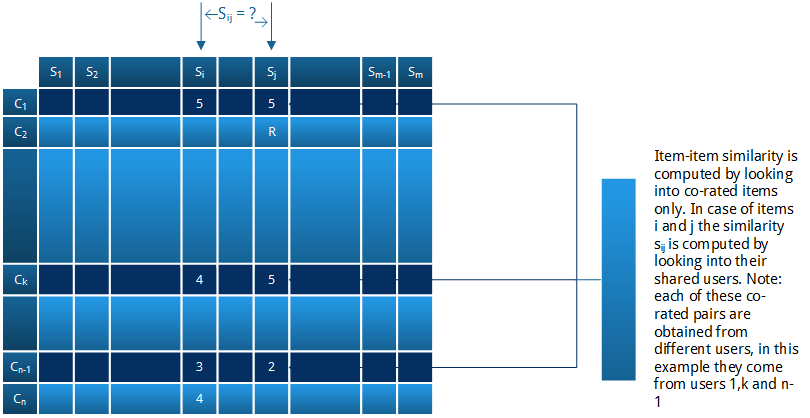
\includegraphics[width=5in]{image/itemsim.png}
    \centering
    \caption[Item-item similarity]{Item-item similarity}
    \label{figure:itemsim}
\end{figure}

There are a number of ways of computing the similarity between items. E.g. by
means of cosine-based similarity. In this case, two items are though of as two
vectors in an $C$ dimensional user space. The similarity between the items is
found by computing the cosine of the angle between the two vectors.

\begin{equation}
sim(s',s) = cos(\vec{s'},\vec{s}) = \frac{\vec{s'} \cdot \vec{s}}{\|\vec{s'}\|^{2} * \|\vec{s}\|^{2}}
\end{equation}

The item similarities can then used to find the Top-N recommendations. Each
user has a set of items $S_{c}$ previously rated by the user which we want to
compute top-N recommendations for. First, we identify the set $C$ of candidate
items recommended items by taking the union of the $k$ most similar items and
removing each of the items in the set $S_{c}$ the user already has rated; then
calculate the similarities between each item of the set $C$ and the set
$S_{c}$, using only the $k$ most similar items for each item in $S_{c}$. The
resulting set of items in $C$ are sorted in descending order of similarity and
will be the recommended as the item-based Top-N list \cite{Karypis2001}.

\subsubsection{Model-based Methods}


As the name implies, Model-based approaches provide recommendations by first
developing a model of the user ratings, which is then used to make predictions.
These algorithms develop a model of user ratings rather than identify a
neighborhood of similar users or items. These models can be built using various
strategies, such as Singular Value Decomposition (SVD), Principal Component
Analysis (PCA), Rule-based Strategies, Clustering Strategies and Bayesian
Networks.

Latent factor models is probably the most representative approach. Latent
factor models transform both items and users to a latent factor space. The
latent factor space tries to explain the ratings by characterizing both items
and users on factors automatically inferred from the data. The most popular
latent factor models are based on matrix factorization techniques
\cite{Koren2009}.

The main idea behind matrix factorization is just as its name implies,
factorize a matrix, finding two or more matrices such that when you multiply
them you get back the original matrix. Matrix factorization can be used to
discover latent factors underlying the interactions between the users and
items. These factors \emph{explain} how a user rates an item (i.e. that a user
would give high ratings to a certain shirt if he likes the brand, or if the
color is nice). If we can discover these factors, we should be able to predict
a rating with respect to a certain user and a certain item based on the
correlation between their factors.

A matrix factorization model map both users and items to a joint latent factor
space of dimensionality $f$, where $f$ is the number of latent factors. The
number of latent factors are usually determined by using a hold-out dataset or
cross-validation by evaluating the prediction error experimenting with
different values. It is also worth mentioning that this in some ways can be
seen as a trade-off between model building complexity and accuracy as having
more features makes the model building more expensive. Each user $c$ is
associated with a vector $p_{c} \epsilon \mathbb{R}^{f}$, and each item $s$ is
associated with a vector $q_{s} \epsilon \mathbb{R}^{f}$. Giving us a matrix Q
containing the user factors and a matrix P containing the item factors as
exemplified in Figure \ref{figure:matrixdecomp}.

\begin{figure}[H]
    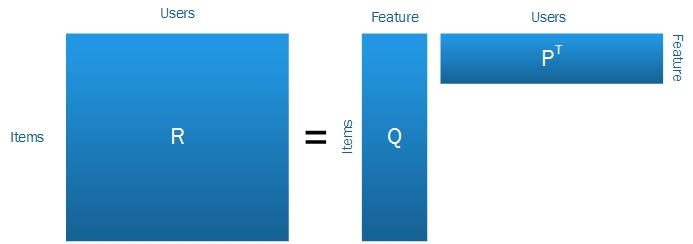
\includegraphics[width=5in]{image/matrixdecomp.jpg}
    \centering
    \caption[Matrix decomposition of the rating matrix $R$]{Matrix decomposition of the rating matrix $R$}
    \label{figure:matrixdecomp}
\end{figure}

User-item interactions are modeled as inner products in that space. For a given
item $s$, the elements of $q_{s}$ measures the extent to which the item
possesses those factors, positive or negative. Likewise, for a given user $c$,
the element $p_{c}$ measures the extent of interest that user has in items that
are high on the corresponding factors. The resulting dot product $\hat{u(c,s)}$
captures the overall interest of the user in the characteristics of the items.

\begin{equation}
u(c,s) = p_{c}^{T}q_{s} = \sum_{k=1}^{f} q_{sk}p_{kc}
\end{equation}

The problem then, is to discover the user factor matrix $P$ and the item factor
matrix $Q$ such that their product approximates the original rating matrix $R$.

\begin{equation}
R \approx Q \times P^{T} = \hat{R}
\label{equation:dotproduct}
\end{equation}

To learn the factor vectors the system minimizes the regularized square error
on the set of known rating $K$.

\begin{equation}
\label{equation:minimize}
min_{q, p} = \sum_{(c,s)\epsilon K} (u(c,s) - p^{T}_{c}q_{s})^{2} + \lambda ( \Vert q_{s} \Vert ^{2} + \Vert p_{c} \Vert ^{2})
\end{equation}

However, it is important to remember that our goal is generalize beyond the
observed ratings, in a way that we can predict future unknown ratings. The
system should therefore avoid overfitting the data by regularizing the learned
parameters, whose magnitudes are penalized. $\lambda$ controls the extent of
regularization, and much like $f$, often determined by cross-validation. Two
possible approaches to minimizing Equation \ref{equation:minimize} is to use
Stochastic Gradient Descent or Alternating Least Squares \citep{Koren2009}.\newline

Consider the following example where we have the following rating matrix R
shown in Table \ref{table:ratingMatrix} containing the rating of four users $C$
for four items $S$, giving us a $C \times S$ matrix with explicit ratings on a
  scale from 1 to 5.

\begin{table}[!htbp]
    \centering
    \begin{tabular}{|c|c|c|c|}
    \hline
    5.00    & 5.00  & 2.00 & -    \\ \hline
    2.00    & -     & 3.00 & 5.00 \\ \hline
     -      & 5.00  & -    & 3.00 \\ \hline
    3.00    & -     & -    & 5.00 \\ \hline
    \end{tabular}
    \caption{Rating matrix R ($C \times S$)}
    \label{table:ratingMatrix}
\end{table}

Given that $f = 3$, we might end up with the following matrix $P$ and $Q$

\begin{table}[!htbp]
\centering
\begin{tabular}{|c|c|c|}
\hline
1.81    &1.62   &0.74\\ \hline
2.66    &1.71   &-1.08\\ \hline
1.73    &-0.23  &0.78\\ \hline
3.16    &-0.24  &0.90\\ \hline
\end{tabular}
\label{table:ItemFeature}
\caption{User factor matrix $P$ ($C \times f$)}
\end{table}

\begin{table}[!htbp]
\centering
\begin{tabular}{|c|c|c|c|}
\hline
1.12    &   1.49    &   0.48\\ \hline
1.31    &-0.52  &0.59\\ \hline
1.13    &0.67&  -0.52\\ \hline
1.39    &0.05&  0.45\\ \hline
\end{tabular}
\label{table:UserFeature}
\caption{Item factor matrix $Q$ ($S \times f$)}
\end{table}

Equation \ref{equation:dotproduct} then gives us the following rating prediction matrix $\hat{R}$.

\begin{table}[!htbp]
\centering
\begin{tabular}{|c|c|c|c|}
\hline
4.79    &5.01   &1.97   &3.61 \\ \hline
1.97    &1.96   &2.85   &4.80 \\ \hline
2.75    &4.71   &1.40   &2.94 \\ \hline
2.93    &3.30   &2.74   &4.78 \\ \hline
\end{tabular}
\label{table:PredictionMatrix}
\caption{Rating prediction matrix $\hat{R}$}
\end{table}

As you can see the values of known ratings in Table \ref{table:ratingMatrix}
are fairly similar to the corresponding ratings in the rating prediction
matrix.

\subsection{Hybrid approaches}

A term \emph{hybrid recommender systems} is used to describe any recommender
system that combines multiple recommendation techniques together to provide
recommendations. Burke et al. \cite{Burke2002} identified seven different
classes of hybrid recommender systems:

\begin{itemize}
\item Weighted: The score of different recommendation components are combined numerically.
\item Switching: Switching between recommender systems depending on the situation.
\item Mixed: Recommendations from different recommenders are presented together.
\item Feature Combination. Features derived from different knowledge sources
are combined together and given to a single recommendation algorithm
\item Feature Augmentation: One recommendation technique is used to compute a
feature or set of features, which is then part of the input to the next
technique.
\item Cascade: Recommenders are given strict priority, with the lower priority
ones breaking ties in the score of the higher ones
\item Meta-level: One recommendation technique is applied and produces some
sort of model, which is then the input by the next technique
\end{itemize}

Most commonly hybrid systems are built by combining collaborative and
content-based methods in an attempt to mitigate the limitations the approaches
suffer individually. Adomavicius and Tuzhilin \cite{Adomavicius2005} lists the
following approaches to building hybrid recommender systems:

\begin{itemize}
\item Implementing the systems separately and combining their predictions
\item Incorporating content-based characteristics into a collaborative approach
\item Incorporating collaborative characteristics into a content-based approach
\item Constructing a general unifying model that incorporates both
content-based and collaborative characteristics
\end{itemize}

\subsection{Recommender System Challenges}

Below we briefly mention some of the main challenges one faces when working
with recommender systems.

\subsubsection{Scalability}

As the number of existing users and items blow up, traditional CF algorithms
suffer serious scalability problems. The model building phase of \emph{Traditional}
collaborative filtering methods have a complexity of O(MN) where $M$ is the number
of users and $N$ is the number of items. For systems with millions of users and items,
even a complexity of $n$ is too large. Another fundamental issue is how to embed the
core recommendation techniques in real operational systems and how to deal with massive
and dynamic sets of data produced by the interactions of users with items. Recommender
systems are expected in many cases to provide rapid recommendations online, it is
therefore also important to consider how fast the system provides recommendations.

Better scalability and improved accuracy make the item-item collaborative filtering
approaches more favourable in many cases. The computational complexity of item-to-item
based algorithms are up to two orders of magnitude faster than traditional user-based
algorithms \cite{Deshpande2004}. Dimensionality reduction techniques such as
SVD can deal with the scalability by providing more compact representations and
quickly produce good recommendations. However, most dimensionality reduction
techniques must undergo expensive matrix factorization steps.

\subsubsection{Sparsity}

In practice, many recommender systems deal with very large item collections.
This means that the number of ratings obtained is usually very small compared to the
number of ratings that it needs to predict. Efficient prediction of ratings from a small
number of examples is therefore important. The \emph{reduced coverage} problem
occurs when the number of users' rating may be very small compared to the number of items.
This may lead to that the recommender is unable to provide recommendations for a large
portion of the items. \emph{Neighbour transitivity} refers to the problem in which users
with similar tastes may not be identified due to a lack of co-rated items, making
collaborative filtering futile, since it relies on comparing users to predict unknown ratings.

\subsubsection{Cold-start}

Conceptually, the cold-start problem can be viewed as a special instance of the
sparsity problem, where most elements in a certain row or column are zero. The
cold-start problem further emphasizes the importance of the sparsity problem.
Whenever a new user or item enters the system, it is difficult to find similar
ones as there is little or no information available. New items can therefore
not be recommended until they have been recommended by a substantial amount of
users. Similarly, giving \emph{good} personalized recommendations to new users
based on a few ratings is difficult, since it does not give a good overall
picture of a users tastes and preferences. These problems are known as the
\emph{cold-start user} and \emph{cold-start item} problems.

\subsubsection{Shilling attacks}

In recommender systems where everyone can give ratings, people may give lots of
positive ratings to their own items and negative ratings to their competitors.
It is often necessary for collaborative filtering systems to introduce
precautions to discourage such kind of manipulation.

\subsection{Terminology}

%TODO - Any more RS related terminology that needs explaining?

\subsubsection{Explanations / Transparency}

Tintarev et al. \cite{Tintarev2007} lists seven roles a that can be played by explanations in recommender systems:

\begin{itemize}
\item Transparency: Explaining how the system works
\item Scrutability: Allowing the users to tell the system it is wrong
\item Trust: Increasing user confidence in the system
\item Effectiveness: Help users make good decisions
\item Persuasiveness: Convince users to try or buy
\item Efficiency: Helping users to make decisions faster
\item Satisfaction: Increasing the ease of use or enjoyment
\end{itemize}

In collaborative filtering systems the explanations is of the form "Other users
similar to you liked this item", while in content-based style explanations, the
item's attributes which most affected the item to be recommended to the user
are illustrated. For example, in a fashion recommender, an explanation may be
of the form "This shirt was recommended because it's a Ralph Lauren who you
seem to like".

% !TEX root = ../../report.tex
\section{The Cold-start Problem}

%Can the different approaches be classified? E.g. 3 main categories of approaches
    %Initial categorization
        %Interview process
        %Hybrid approaches
        %Key figures / Seed users
        %Filterbots
        %Trust-aware / Trust propagation

In the literature, the term cold is used about an object in a system, or a
whole system, which is new \cite{Schein2002, Park2006}. Cold-start scenarios in recommender systems are
situations in which little/no prior events, like ratings or clicks, are known
for certain users or items. The cold-start problem can be divided into three sub problems:

\begin{itemize}
  \item \emph{Cold-start system}: A situation where we only have new users and
  little or no ratings for the items.

  \item \emph{Cold-start item}: The problem of recommending items that are new
  to the system, which have not received any ratings.

  \item \emph{Cold-start user}: The problem of giving accurate recommendations
  to a user who is new to a recommender system.
\end{itemize}


For example in a scenario where the average item in an item collection have 5
000 ratings, a new item with only 5 ratings would be considered a
\emph{cold-item}. Likewise, in a recommender system where the average user has
rated 25 items, a user who only has rated 2 items, would be considered a
\emph{cold-user}.

The cold-start system problem is mainly a collaborative filtering problem, and
can be seen as a combination of the cold-start user and cold-start item problem
where the majority of the users are new to the system and have expressed few
preferences, resulting in a very sparse user-item matrix, rendering traditional
collaborative-filtering methods futile. Most traditional algorithms only work
effectively in environments where the datasets has high information density. In
fact, in extreme cases, when data is very scarce, simple non-personalized
recommendations based on global averages can outperform collaborative-filtering
algorithms \cite{Park2006}. The reason why the cold-start system problem is not
so evident in content-based systems is due to \emph{User Independence}, meaning
that the system only exploits ratings provided by the active user to build her
profile. Instead, collaborative filtering methods need ratings from other users
to find the "peers" of the active users.

In content-based systems, new items can easily be recommended using the content
information of the item, making it a popular solution to the \emph{cold-start
item} problem. This problem is more severe in collaborative-filtering systems
where items are only recommendable if they have been rated by substantial
amount of users. New items will therefore not be recommendable before multiple
users somehow stumble upon the new item while e.g. browsing the item
collection, unless additional measures are taken to solve this problem. To
\emph{solve} the new-item problem, there are two commonly used (simple)
solutions often used in E-commerce websites:\marginpar{heri-notes: cite}

\begin{itemize}

\item Advertising at the front-page of the website, putting the new items in an
eye catching position. This solution, however, may this result in that some
users, which don't like these new items, might leave the website.
\item Requesting the user to choose one or more of his/hers categories while
registering for the site, and recommend items from the selected categories.
This approach however, requires active user involvement and complicates the
sign up process. Many users might chose not to give up any personal interest
information, thus the user group covered by this solution could end up not
being large enough.
\end{itemize}

The cold-start user problem is present both in content-based and collaborative-filtering systems.
Since Collaborative Filtering is based on the idea that like-minded users have similar tastes and
preferences, a new user therefore naturally poses a challenge to a CF recommender, since the system has no knowledge about
the preferences of the new user, and can therefore not find any like-minded users. The system must therefore acquire some
information about the new user before it can start making personalized recommendations. In a typical domain, for example
in the domain of books, the number of items is very large (in the order of tens of thousands) while the number of items
rated by every single user is in general small (in the order of dozens or less). This means that it is very unlikely two
random selected users have rated any items in common and hence they are not comparable. The system will therefore most
likely struggle to find users with tastes that are \emph{truly} similar to the target user. Similarly, in content-based
systems, the lack of ratings given by the target user, means that the target user will have a limited content-profile,
since the users content profile is constructed using content-information from his/hers rated items. In both cases,
recommendation quality is most likely bound to suffer.\newline

\marginpar{heri-notes: hvordan kan dette problemet være relevant for oppgaven deres?}

This section will present a few different solutions to the cold-start problem, focusing mainly on \emph{complete} solutions to the cold-start problem.

\subsection{Trust Aware Recommender Systems}

One promising direction to solve the cold-start problem is the incorporation of
a trust network. A trust network can significantly help alleviate the
cold-start user problem, primarily since the trust statements between users can
be propagated and aggregated, and consequently connect more people and
products. By making clever connections in the trust network, newcomers can
immediately gain access to a wide range of connections.

%Due to the popularity of social networks such as Facebook, more and more
%researchers turn to incorporate the social relationships (e.g. trust) of users
%to help complement users’ preference in addition to item ratings, in order to overcome the limitations of existing recommender systems

For example, when looking for movie recommendations we often turn to our friends which we share a similar taste in movies with. Trust can be defined as: "believe in the reliability, truth, or ability of", and in the context of recommender systems a trusted user would be a user you trust to provide you with good recommendations. E.g. in the case of the Epinions dataset \cite{Epinions}, users can explicitly state whether they trust or distrust a user [1, -1], i.e. reviewers whose reviews and ratings they have consistently found to be valuable or reviewers which they find consistently offensive, inaccurate or not valuable. In decentralized environments where everyone is free to create content and there
is no centralized quality control entity, evaluating the quality of the content becomes an important issue. This phenomenon can be observed in online
marketplaces such as E-bay where users can create "fake" auctions and in peer-to-peer networks where peers can enter corrupted items. In these environments, it is often a good strategy to delegate the quality assessment task to users themselves. E.g. \emph{Ebay.com} allows users to express their level of satisfaction after every interaction with another user. Trust relationships of users are often employed in order to correlate more potential raters for the active users who require recommendations \cite{Massa2004, Massa2007}. Massa et. al. \cite{Massa2004} also show that some of the weaknesses of recommender systems such as data sparseness and their susceptibility to shilling attacks could be alleviated by incorporating trust.

% The formals
In \cite{Massa2004}, Massa et al. proposes a Trust-Aware recommender system
architecture.  To capture all the trust statements we need a $CxC$ matrix,
where $C$ is the number of users, since each user is allowed to express a trust
value in every other user. This matrix will make up our trust network among the
users. If $u$ trusts $v$, then there is a value $t_{u,v}$ for this trust which
is a real number in $[0,1]$. Zero means no trust and one means full trust. This
additional information can be organized in a trust network and a \emph{trust
metric} can be used to predict the trustworthiness of other users as well (for
example, friends of friends). The idea here is to not search for similar users
as CF does but to search for trust-able users by exploiting trust propagation
over the trust network. The items appreciated by these users are then
recommended to the active user.

% Web of Trust - Figure explanation
Consider the example shown in Figure \ref{figure:weboftrust}. User $A$ has
issued a trust statement in $B$ and $C$; hence $B$ and $C$ are in the web of
trust of $A$. Using these explicit trust statements, it is possible to predict
trust in unknown users by propagating trust, making it possible to infer
something about how much user $A$ could trust $D$.

\begin{figure}[H]
    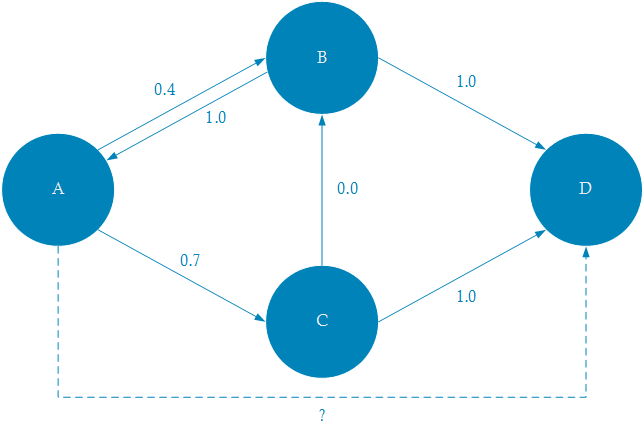
\includegraphics[width=2in]{image/webofTrust.png}
    \centering
    \caption[Trust Network]{Trust Network. Nodes are users and solid edges are trust statements. The dotted edge is one of the undefined and predictable trust statements (Adopted from \cite{Massa2004})}
    \label{figure:weboftrust}
\end{figure}

In addition to the trust network we will also have a rating matrix of size
$CxS$, where $S$ is the number of items. This rating will not differ from a
standard rating matrix, which are used in traditional collaborative filtering
systems. The value $u(c,s)$, is the rating given by user $c$ to item $s$, the
rating scale may differ from system to system.

% Architecture
The systems takes as input the trust network and the ratings matrix and
produces, as output, a matrix of predicted ratings that the users would assign
to the items. Figure \ref{figure:trustarchictecture} shows a conceptual
overview of the trust-aware recommender system architecture.

\begin{figure}[H]
    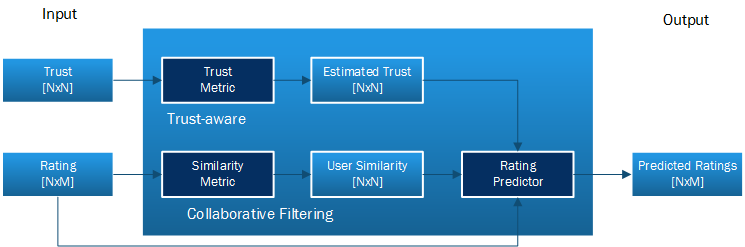
\includegraphics[width=5in]{image/trustawarearchitecture.png}
    \centering
    \caption[Trust-Aware Recommender System Architecture]{Trust-Aware
    Recommender System Architecture (Adopted from \cite{Massa2004})}
    \label{figure:trustarchictecture}
\end{figure}

The \emph{Trust Metric} module takes the trust network as input, and exploits
trust propagation in order to predict, for every user, how much she could trust
other users. Trust metrics can either be local and global. Global trust metrics
produces an estimated trust matrix with all the rows equal, meaning that the
estimated trust in a certain user (column) is the same for every user (row). A
simple local trust metric could e.g. for each user assign to every other user a
predicted trust based on her minimum distance from the source user. More
sophisticated ones could also be employed. If we again consider Figure
\ref{figure:weboftrust}, we could employ a local trust metric where the
predicted trust is based on the minimum distance from the source user. If we
set the maximum propagation distance $d$, a user at distance $n$ from the
source user will have a predicted trust value of:

\begin{equation}
t_{u,v} = \frac{d-n+1}{d}
\end{equation}

Giving users not reachable within the maximum propagation distance a trust of
$0$. Using user $A$ as the source user, the users at distance $1$ ($B$ and $C$)
would get a trust value of $(4-1+1)/4 = 1$, while the user at distance 2 (D)
would get a predicted trust value of $(4-2+1)/4 = 0.75$. Meaning that we will
have a linear decay in trust based on the distance from the source user.

Massa et al. \cite{Massa2007} experimented with both local and global trust
metrics. They used the PageRank algorithm as a global trust metric. PageRank
tries to infer the authority of every single user by examining the structure of
the network. The algorithm follows a simple idea: if a link from user $A$ to
user $B$ represent a positive vote casted by $A$ to $B$, then the global rank
of a page depends on the number (and quality) of the incoming links. The trust
values assigned by users to users are used to predict the trustworthiness of
unknown users. Their findings, not surprisingly, indicate that Global Trust
Metrics are not suited for the task of finding good neighbours, especially for
providing personalized recommendations, but is more suited to applications such
as \emph{Ebay.com} to find untrustworthy users. As a local trust metric they
used MoleTrust, which is a depth-first graph walking algorithm with a tuneable
trust horizon which allowed them to experiment with different propagation
distances. They found trusted users to be good predictors. For the cold-start
users they achieved a MAE of 0.674 when looking at friends of friends, compared
to traditional collaborative filtering which scored 1.094. The difference is
very high, and particularly relevant as it is important for recommender systems
to generate personalized recommendations as soon as possible for new users, so
that these users appreciate the system and keep using it.

The \emph{Similarity Metric} module computes the user similarities, this is one
of the standard steps of any traditional collaborative filtering technique,
user similarities can be found e.g. by using the Pearson Correlation
Coefficient. The intuition is that, if a user rates in a similar way to another
user, then her ratings are using for predicting the ratings for that users.

The \emph{Rating Predictor} can use the neighbours from the user similarity
matrix, the estimated trust matrix or a combination of both in order to
calculate the predicted ratings.

% Using a Trust Network to Improve Top-N Recommendation

Jamali et al. \cite{Jamali2009} propose two different methods for getting
around the cold-start user problem using a trust network. Their first approach
called \emph{Random Walk} only utilize the trust network to provide
recommendations. Starting from the active user $u$, we perform a random walk on
the trust network. Each random walk stops at a certain user. Then the items
rated highly by that user will be considered as recommended items, ordered
according to the ratings expressed by that user. Several random walks are
performed to gather more information and compute a more confident result. The
estimated rating of each item is the average of ratings for that item over all
raters considered. At the end, we output items with the highest estimated
rating as top-N recommended items. Their second approach called \emph{Combined
Approach} uses both user-user similarities and the trust network to provide
recommendations. In this approach we compute the top $K$ trusted users in the
network and rank the items rated by these trusted users to compute top-N
recommended items. The top $K$ trusted users can either be found by
\emph{Breadth First Search} or \emph{Random Walk in the social network}. We use
the collaborative filtering approach to compute another set of top-N
recommended items. Finally, we merge these two lists to produce a combined list
of top-N recommended items. Items returned by CF is denoted as $CF_{u}$, while
the items returned by Trust-based approach are denoted $TR_{u}$.

\begin{equation}
 \hat{u}(c,s) =
  \begin{cases}
   \frac{u_{tr_{c,i}}+u_{cf_{c,i}}}{2}     & i \in TR_{u};i \in CF_{u}         \\
   \hat{u_{tr_{c,i}}}                      & i \in TR_{u};i \not \in CF_{u}    \\
   \hat{u_{cf_{c,i}}}                      & i \in CF_{u};i \not \in TR_{u}     \end{cases}
\end{equation}

The top-N items with the highest value of $\hat{u}(c,s)$ will be returned as
the top-N recommended items. The authors also experimented with weighted
averaging in the case where the item appear in both $TR_{u}$ and $CF_{u}$.

The top-N items with the highest value of $\hat{u}(c,s)$ will be returned as
the top-N recommended items. The authors also experimented with weighted
averaging in the case where the item appear in both $TR_{u}$ and $CF_{u}$.
Their approaches showed great improvements in recall for cold-start users,
improving the performance by 50\% over standard CF methods. The main
improvements however, are the coverage of the trust-based approaches, while
still maintaining the same or even slightly better precision than the standard
CF methods.

% Trust-aware Recommender Systems + Trust-Aware Collaborative Filtering for Recommender Systems
% Article Comments:
%   Requires user involvement (explicitly express trust) - is this a acceptable?

%Massa et al. \cite{Massa2004, Massa2007} propose using trust information
%explicitly expressed by the users. Users are allowed to state how much they
%consider every other user trustworthy that, in the context of recommender
%systems, is related to how much they consider the ratings provided by a certain
%user valuable and relevant.

% Alleviating the Sparsity Problem of Collaborative Filtering Using Trust Inferences
% Article Comments:
%   - Pretty good general model for dealing with sparsity
%   - Requires no additional information such as product details, demographic information about userstrus


Papagelis et al. \cite{Papagelis2005} proposed to alleviate sparsity using
trust inferred from user-user similarity. This approach does therefore not
require users to explicitly express their trust in other users, unlike the
approaches described above, the trust information is inferred from the
underlying social network of the rating matrix. Their approach is based on the
assumption that the more similar two users are, the greater their established
trust would be considered.

\begin{figure}[H]
    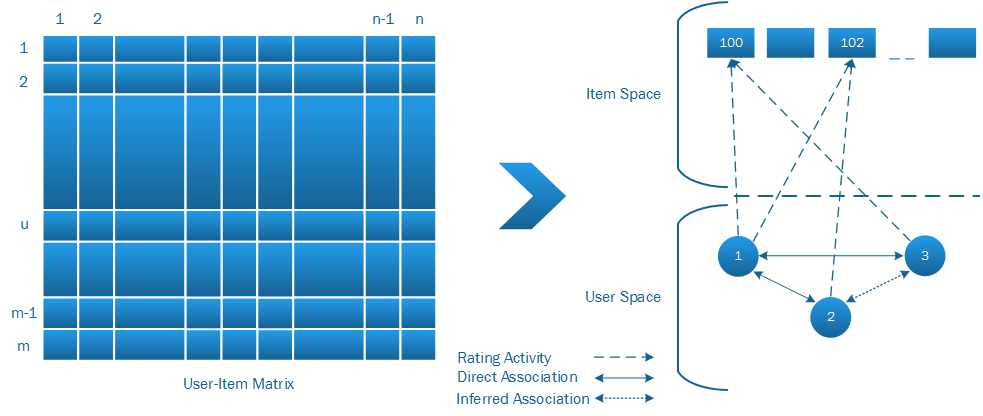
\includegraphics[width=5in]{image/trustnetwork.png}
    \centering
    \caption[Underlying Social Networks in Recommender Systems]{Underlying Social Networks in Recommender Systems}
    \label{figure:cfsocialnetwork}
\end{figure}

Due to the number of ratings that exist in recommendation systems, underlying
social networks are very sparse. There are cases in which insufficient or loss
of information is detrimental for the recommendation algorithms. Consider
Figure \ref{figure:cfsocialnetwork}, classic CF will associate only the users
which have co-rated an item (User $1$ and $2$ and user $1$ and $3$). To deal
with the problem of a sparse social network, it is possible to infer trust
between a source user $S$ and a target user $T$ through an intermediate user
$N$ (User $2$ and $3$ are connected through the intermediary user $1$), as
shown by the \emph{Inferred Association} arrow. According to this process,
trust is propagated in the network and associations between users are built,
even if they have no co-rated item. Trust paths can be of variable length,
depending on the number of associations that one needs to traverse in order to
reach the target user.

% Trust-paths
For example, if the trust $t_{(1,2)} = 0.7$ based on 5 co-rated items
and $t_{(1,3)} = 0.35$ based on 2 co-rated items, then the trust
between user $2$ and $3$ through $1$ is, $\frac{0.7*5}{5+2} + \frac{0.35*2}{7} = 0.6$.

In order to express the subjective notion of trust, the authors set up a
confidence model that is assigned to each direct association of the network
that expresses the reliability of the association. Confidence is related to the
number of co-rated items between two users. The confidence scores are all
expressed in relation to the most confident association for each user.

\begin{equation}
c_{(s,t)} = \frac{n(I_{s} \cap I_{t})}{n(I_{s} \cap I_{u_{MAX_CONF}})}
\end{equation}

Using the above example, assuming that the maximum number of co-rated items
user $1$ has with any user is 7, $c_{(1,2)} = \frac{5}{7}$.

% Results/Findings
The authors achieved improved accuracy for all sparsity levels. With a sparsity
level of $99.9\%$ the 2-HOP CF (friend of friends) increased the MAE
performance by $17\%$ over standard CF methods.

%TODO - READ: A Matrix Factorization Technique with Trust Propagation for Recommendation in Social Networks
%Jamali et al. propose a technique for incorporating trust using matrix factorization, called SocialMF.
%Leverage regularization model to fusing the one mode data by minimizing the gap between the taste of a user and the taste of her trusted friends
%In their model, the users which have not expressed any ratings feature vectors will be learned to be close to their trusted neighbors.

Victor et al. \cite{Victor2008} points out that cold-start users not only have
expressed few ratings, but also typically have expressed trust in few users. In
order for trust-aware recommenders to help cold-start users they need to have
expressed trust in atleast one user. But choosing who to connect to is often a
difficult task. To help cold-start users find trusted users, Victor et al.
propose using key figures or mavens (users who write many reviews), frequent
raters (users who evaluate many items) and connectors (users with
many trust connections). By connecting to these key figures, cold-start users
shown a significant increase in coverage while still maintaining good accuracy.
They also show that connecting to key figures are more beneficial to a
cold-start user than connecting to a random user.

\subsection{Filterbots}

% Na¨ıve Filterbots for Robust Cold-Start Recommendations

Park et al. \cite{Park2006} propose using filterbots to improve the cold-start
performance of collaborative filtering methods. Their filterbots are a varition
of RipperBots, described in detail in \cite{Good1999}. A filterbot is an
automated agent that rates all or most items using information filtering (IF)
techniques. The filterbots injects psuedo users or bots into the system. These
bots rate items algorithmically according to item features and user profiles.
For their movie recommendation systems the authors used 7 global bots which
e.g. rated movies based on average item rating, a critic bot that generates ratings
based on the average critic (pre-selected users) ratings, an award bot that
generates rating based on the awards a movie has won, and so on. These ratings
generated by these bots are injected into the user-item matrix along with
actual user-item ratings. Standard CF algorithms are then applied to generate
recommendations.

Their approach clearly demonstrated better robustness to all three cold-start situations than standard item-based
and user-based collaborative filtering. The improvements were most evident on
the datasets with a high degree of sparsity.

\subsection{Wisdom of the better few / Seed users}

% Wisdom of the Better Few: Cold Start Recommendation via Representative based Rating Elicitation

Liu et al. \cite{Liu2011} propose an approach in which they elect a few
representative users and items. The representative set should represent a set
of active users or items who well represent the entire population but with
little taste overlap. In their approach they wish to find a rank-k
factorization of the form $Y \approx XR$ or $Y \approx CX$ where $X$ is a
loading matrix consisting of free parameters and $R$ and $C$ which is the
component matrix consisting of actual rows or columns from $Y$. The
representative users and items are found using dimensionality reduction
techniques by reducing the column space of the rating matrix from $m$ to $k$.
And then applying basis selection based on the maximum-volume principle to
select the $k$ most representative users or items. In order to be able to
recommend new items to the users it must first be rated by the $k$
representative users, likewise for new users to be rated they need to rate the
$k$ most representative items. Their method therefore easily allows new users
and items to be \emph{folded in}.

\subsection{Intelligent Selection / Interview Process}\mbox{}\\

\begin{chapquote}[30pt]{Vanessa Redgrave}
  "Ask the right questions if you're going to find the right answers"
\end{chapquote}

% Getting to Know You: Learning New User Preferences in Recommender Systems

As pointed out by Rashid et al. \cite{Rashid2002}, the most direct way of
acquiring information for use in personalized recommendations from a new users
is to present item for the user to rate. However, they argue that the system
must be careful to present useful items to garner information. A food
recommender should probably not ask whether a new user likes vanilla ice cream
since most people like vanilla ice cream. Therefore, knowing that a new user
likes vanilla ice cream tells you very little about the user. The choice of
what questions to ask a new user, then, is critical. The authors performed a
study of different item selection strategies that collaborative filtering
recommender systems can use to learn about new users. They presented the users
with a questionnaire with items asking them to rate/select the ones they like.
Their strategies can be divided into five classes, which they evaluated based
on user effort and accuracy:

\begin{itemize}
\item \emph{Random:} strategies: Strategies that avoid bias in the presentation
of bias
\item \emph{Popularity:} Select among the top N items where the probability
that an item is selected is proportionate to the items popularity.
\item \emph{Pure entropy:} Present the items with the highest entropy that the
user has not seen
\item \emph{Balanced strategies:} A balanced approach combining both popularity
data and entropy.
\item \emph{Personalized:} As soon as some information is known about a user,
present items specifically tailored to that user using e.g. item-item
similarity
\end{itemize}

The authors found Popularity and balanced strategies to perform the best. Their
recommendation for an e-commerce recommender is to start recommending the most
popular items, rather than the highest rated ones, and then use item-item
strategies to personalize the recommendations as quickly as possible. This
study was later extended by Rashid et al. \cite{Rashid2008} where they more
closely examined information theoretic strategies for item selection. In the
article they introduced three new strategies, which again was evaluated based
on user effort and accuracy:

\begin{itemize}
\item \emph{Entropy0}: Entropy Considering Missing Values
%\item \emph{HELF:} Harmonic mean of Entropy and Logarithm of Frequency
\item \emph{IGCN:} Information Gain through Clustered Neighbors
\end{itemize}

The authors point out that approaches like popularity is likely to worsen the
\emph{prefix-bias}, meaning that popular items garner even more evaluations.
The accuracy differences between the approaches is fairly small, IGNC performed
the best closely followed by Entropy0 and Popularity. However, the expected
utility of the profiles built using popularity is much lower than the
information theoretic approaches.\newline

% User effort vs. accuracy in rating-based elicitation
The question then, is how many items you should ask a user to rate. Cremonesi
et al. \cite{Cremonesi2012} performed a set of experiments where they looked
at the trade-off between user-effort and accuracy. More specifically, how many
ratings are enough to provide good quality recommendations to new users? The
authors conclusion is that between 5 and 20 ratings are optimal for the movie
domain. They concluded that 10 ratings is \emph{enough}, but that this number
depends on the recommendation method and the dataset used.

\subsection{Hybrid Methods}

%TODO - Add some fancy math, wait until matrix factorization intro is in place (so we do not mess up notations)
%TODO - Find some sweet cf articles incorporating demographic information

Another line of search for solving the cold-start problem is to utilize
features of items and users. The content features can be used to capture the
similarities between users and items, thus reducing the amount of data required
to make accurate predictions. User data that may be collected typically
includes age, gender, nationality, marital status, income, educational level
and occupation. Item data could e.g. be the price of a product, title,
description, editorial ratings and so. The idea is that people with a more
common background share a more similar taste than someone with a random
background, and therefore good recommendations can be made as long as we know
something about the new user's background.

This section will present some latent factor models presented recently proposed
that incorporate both user/item features in addition to user-item interactions.
In Matrix factorization methods, the regularization is mostly based on a
zero-mean Gaussian prior on the factors, we refer often referred to as
ZeroMean. However in the following models the dyadic response matrix $Y$ is
estimated by a latent factor model such that $Y \approx U^{T}V$, where the
latent factor matrices, $P$ and $Q$, are estimated by regression such that $P
\approx FX$ and $Q \approx MZ$. $X$ and $Z$ denote user attribute and item
feature matrices, and $F$ and $M$ are weight matrices learned by regression.
The main difference between the following methods is how they estimate these
weight matrices.

% Regression-based Latent Factor Models

Agarwal et al. \cite{Agarwal2009} propose a class of latent factors models
called regression-based latent factor model (RLFM) that incorporates both
user/item features and past interaction data into a single model. Their
approach utilizes features of items and users as the prior distribution for
latent profiles in matrix factorization. Regularizing latent factors through
regression has important consequences when modeling sparse dyadic data. For
users/items with little data, one obtain reliable factor estimates by using the
regression estimates as a fallback. This allows the model to effectively deal
with both cold start and warm start situations. Their method assumes a Gaussian
prior, but replaces the zero mean with a feature-based regression, thus it
simultaneously regularizes both user and item factors through known features.
Users and items are anchored around a global feature-based one where profiles
are constructed by estimating deviations from the global ones in a smooth
fashion. The deviation depends on the amount of information available, e.g.
items/users with sparse data are aggressively "shrunk" to the global one. New
items and users start out with profiles based on their known features that gets
refined smoothly with the availability of more data. The model also supports
dynamic updates, which gives more weight to recent data. Their proposal is a
batched online learning scheme which updates the model on fixed time intervals
or after a predetermined amount of new observations have been made.

Their model outperformed all other models on both the MovieLens and EachMovie
datasets, and their dynamic model in particular significantly outperformed all
other models.

% fLDA: Matrix Factorization through Latent Dirichlet Allocation

Agarwal et. al \cite{Agarwal2010} propose a Matrix factorization method to
predict ratings in recommender system applications where a "bag-of-words"
representation of item meta-data is natural. Their method regularizes both user
and item factor simultaneously through user features and the bag of words
associated with each item. The key idea of their method is to let user factors
take values in an Euclidean space of existing factorization models, but assign
item factors through a richer prior based on Latent Dirichlet Allocation (LDA).
The main idea behind LDA is to attach a discrete latent factor to each word of
an item that can take $K$ different values ($K$-topics) and produce item topics
by averaging the per-word topics in the item. An article where 80$\%$ of the
words are assigned to politics and the rest to education would be though of as
a political article related to the issue of education. This allows us to model
the affinity between user $i$ and item $j$ as $s'{j}\hat{z_{j}}$, where
$\hat{z_{j}}$ is the multinomial probability vector representing the soft
cluster membership score of of item $j$ to the $K$ different latent topics.

% Matchbox: Large Scale Bayesian Recommendations
%   Online algorithm

Stern et al. \cite{Stern2009} presents a probabilistic model called Matchbox.
The system makes use of content information in the form of user and item
meta-data in combination with collaborative filtering information from previous
user behaviour in order to predict the value of an item for a user. Much like
\cite{Agarwal2009} the factors are regularized by incorporating more
flexibility in the Gaussian priors through regression on user and item factors.
Their model is dynamic, meaning that it allows an item's popularity, a user's
taste or user's personal rating scale to drift over time, as well as having the
option to be trained incrementally using Assumed Density Filtering (ADF). This
means that the value of weight matrices $F$ and $M$ will drift over time, this
is accomplished by the addition of Gaussian noise each time step. Inference is
accomplished a combination of message passing and expectation propagation.

The authors show that they can achieve state-of-the-art performance when
training the model in an on-line manner, which is especially beneficial for
dynamic domains where it is important to always have an up to date model.
Matchbox was able to train the model for the Netflix Dataset in about 2 hours
using 8 cores, meaning that it is able to add up to 14000 ratings per second.
These methods also provide quick recommendations, which is important in an
online applications, the system was able to generate 2,500,000 recommendations
in 0.25 seconds using Approximate KD Trees.

% Learning Attribute-to-Feature Mappings for Cold-Start Recommendations
%   Model for positive implicit feedback!
%   Demonstrates usefulness for new-item recommendations
%   See A. Item Recommendation from Implicit Feedback in the article for implicit feedback recommendations
%   k-NN worked best with MORE features than the linear mapping functions
%   Code can be found at: ismll.de/mymedialite

Gantner et al. \cite{Gantner2010} propose a method on how to map additional
information such as user and item features to the latent features of a matrix
(or higher dimensional) factorization model. At the core of their approach is a
standard factorization model, optimized to the recommendation task. The
extensions include a mapping function that compute adequate latent
representations for new entities from their attribute representations. This
mapping function could allow new items and users latent features to be found
only based on content-information and further on be used as if they were
normally trained latent features. The training of the factorization model with
a mapping extension consists of the following steps:

\begin{enumerate}
\item Training the factorization model using the data $S$, and then
\item Learning the mapping functions from the latent features of the entities
\end{enumerate}

The authors use BPR-MF, a matrix factorization model based on the Bayesian
Personalized Ranking (BPR) framework as their factorization model. The authors
experimented with two different ways of mapping item/user attributes to the
factor space (Only attribute-to-feature mapping for items are presented in the
article):

\begin{enumerate}
\item k-NN Mapping: Weighted k-NN regression for each factor. Determine the
k-nearest neighbors as the most similar items according to the cosine
similarity of the attribute vectors.
\item Linear Mapping: Each item factor is expressed by a weighted sum of the
item attributes. Suitable parameters for the mapping function is learned by
optimizing the model for the squared error on latent features.
\end{enumerate}

The authors found that linear mapping worked the best, and that their method
yields accuracy comparable to state-of-the-art methods.

\subsection{A Discussion on the Cold-start Solutions}

\subsubsection{Trust-aware recommenders}

%Summarize results
Massa et al. \cite{Massa2007} found trusted users to be good predictors. When
looking at directly trusted users they improved the MAE from 1.094 using
traditional collaborative filtering to 0.674 for cold-start recommendations. By
propagating the trust they were able to drasticly increase the coverage. The
average number of directly trusted users were 9.88, while the average number of
comparable users using the pearson correlation factor was 160.73. Propagating
at a distance of 2 it is possible to reach 399.89 users, increasing it to 3 and
4 respectively it is possible to reach respectively 4,386.32 and 16,033.94
users. Jamali et al. \cite{Jamali2009} got even better results with their
\emph{Trustwalker} approach by combining trust-based and item-based
recommendations. Massa et al. \cite{Massa2004} also argue that it is more
useful for a recommender system to ask for one trust statement than asking for
one rating for new users.

%How can this be implemented in our system?
Requiring users to explicitly express trust, is not something users necessarily
will frown upon. Services like Instagram, Facebook and many others offers a
\emph{follow} function to their users, filling their news feeds with content from
the users which they have chosen to follow. For SoBazaar we imagine that you
e.g. could chose to follow people either because they have a good taste in
clothes or that you simply are friends, and you want to keep up with what your
friends are buying. We imagine the \emph{follow user} functionality, that has
not yet been implemented, could be used to collect the trust statements. We
believe that trust aware recommender systems is something that should be looked
into at a later point when this functionality is in place, to further enhance
the recommendation quality.

%Scalability & Final Verdict
Propagating trust is expensive. The trust propagation must be computed in
addition addition to the user-user or item-item similarities, and it therefore
scales worse than collaborative filtering methods. It is however, a good general model for
sparsity and increasing robustness of recommender systems, with the downsides
being scalability challenges and the added complexity to the system.

\subsubsection{Interview Process}

%Summarize results
Rashid et al. \cite{Rashid2008} got the best results using information
theoretic approaches and argues that simpler methods such as most popular is
likely to worsen the prefix bias. The authors found Information Gain through
Clustered Neighbours (IGCN) to have the best performance overall, which scored
5 out of 5 stars for accuracy, and would be a good candidate to find items for
the user to rate.

%How can this be implemented?
Our rational behind including these articles is that we envision a simple "hot
or not" tinder like interface to be used to present items to new users when the
first log in to the system. And then ask new users that download the app to
rate e.g. 10 items when first logging in. It is worth mentioning that the
authors of these articles mainly worked on a solution to the cold-start new
user problem. The user-effort dimension of their evaluation could also largely
be ignored as they made a system for movie recommendations. The implications of
this is that a user must have watched a movie, in order to rate it. This is not
as important for the fashion domain, as taking a quick look at an item should
be sufficient to like/dislike it, so we should give more weight to the accuracy
of the system after the interview process than user effort. It is also worth
noting that calculating entropy using implicit ratings is tricky, since the
rating distribution does not range from dislike to like. We can therefore not
find \emph{high-entropy} or \emph{controversial} items which users either tend
to like or dislike, as we have no data about items users dislike.
We are also currently constrained to unobtrusively learn user-profiles from
the natural interactions of users with the system, meaning
that we can not require the user to rate e.g. 10 items before we can start
providing recommendations, as this functionality has not been implemented.

\marginpar{Discussion on suitedness of implicit ratings for entropy
calculations}.

%Scalability & Final Verdict
The scalability of the approach is also fairly good. It requires another module
in addition to collaborative filtering which is used in the non-personalized
step until the user have rated a predetermined amount of items. When enough
items have been rated the CF algorithm is used to produce recommendations. We
really like this approach as it is simple and elegant. Given that a information
theory approach is used this would be a good model for dealing with sparsity,
as the number of ratings would sky-rocket in addition to having ratings for a
large portion of the item collection (not only limited to the most popular
items). The negative aspects of this approach is mainly limited to the fact
that it requires active user involvement.

\subsubsection{Seed users}

In our opinion, this approach is not that suited for our domain, as it fairly
dynamic and we are working with a large item collection. For an item to be
recommendable it must be rated by all representative users, which is highly
unlikely given the size of the item collection itself. E.g. if we have 15
representative users and a spring collection launches containing 6000 items,
for all these items to be recommendable these 15 representative users must rate
all these items.

\subsubsection{Filterbots}

%TODO - Summarize results
Park et al. \cite{Park2006} clearly demonstrated the robustness of their Naive
Filterbot compared to item-based and user-based approaches in all three
cold-start scenarios. The results in \cite{Agarwal2009, Agarwal2010} also shows
that the Naive Filterbots performance is very close to the state-of-the-art
latent factor models.

%TODO - How can we implement this in our system?
To incorporate filterbots in our system we would first have to define what
filterbots we wound want to use. We could e.g. use a Brand-bot that calculates
ratings of brands over all users. The rating of a brand is the average rating
of the items of the given brand, which then is injected into the user-item
matrix. It is worth noting that selecting what bots to add to the system and
and coding them would require some engineering effort, and involve some testing
to validate your bots.

%TODO - Scalability & Final Verdict
Park et al. \cite{Park2006} claim that the added computational complexity of
adding seven global bots is almost negligible. The downside of this approach is
the additional engineering effort required and the fact that it's performance
is not on pair with the more sophisticated latent factor methods.

\subsubsection{Hybrid recommenders}

%TODO - Summarize results

Latent factor models are currently the main paradigm within the recommender
system field and are currently considered the state-of-the-art recommendation
methods. The hybrid methods achieved state-of-the-art performance as well as
having good fallback methods based on user and item features to solve the
cold-start problem.

%TODO - How can we implement this in our system?

To implement these recommenders we would first have to select and extract
user-features from Facebook and item-features from our item database. Another
concern of ours is that our dataset is currently to small for latent factor
methods, and is therefore likely to produce sub-optimal results.

%TODO - Scalability & Final Verdict
%   Which of the models are online?
As most latent factor models, model building is expensive. Matchbox and RLFM
have to option of being trained online, which should further could increase the
cold-start performance, as the model always will be up to date. Latent factor
models are also known to provide quick recommendations. These methods combine
state-of-the-art performance, elegant solutions to the cold-start problem
incorporating meta-information as fallback in addition to having the option to
be incrementally trained.

\subsubsection{Summary}

%TODO - Summary of all the methods, what can we use?
\marginpar{helge - I problem statementdelen bør dere definere (uten å bruke foreløpig ikke definerte termer) hva som er ønskede egenskaper, og prioriter disse. Ta igjen dette her. Col-start og user effort må være mest sentralt foreløpig eller? Holder å gi kvalitativ vurdering (type +/- eller ++/+/-), så fravær av sammenlignbare forsøk virker ikke viktig på meg. Domenet er for spesielt til at vi kan generalisere ggodt tror jeg}

It is hard to compare the performance of the different methods as they have
experimented with different datasets and evaluation measures...

\marginpar{What are the most important 'attributes' to consider?}
I would also argue that having the option to incrementally update the model is
an important feature to further improve cold-start performance. As having a
model that is already updated will instantly incorporate data about new users
and items.

Compare the models based on the following properties:

\begin{itemize}
    \item Accuracy: How accurate is the method...
    \item Cold-start performance: How well does it handle the cold-start related problems?
    \item Scalability: How well does the method scale for larger datasets
    \item User-effort: How much user involvement is required?
\end{itemize}

\begin{table}[H]
    \centering
    \begin{tabular}{|l|l|l|l|l|}
    \hline
    Method					& Accuracy & Cold-start performance & Scalability & User-effort \\ \hline
    Trust-aware RS 			& 		   & 						& \\ \hline
    Filterbots 				& 		   & 						& \\ \hline
    Seed users 				& 		   & 						& \\ \hline
    Intelligent selection 	& 		   & 						& \\ \hline
    Hybrid Methods 			& 		   & 						&	 \\ \hline
    \end{tabular}
    \caption[Evaluation of cold-start methods]{Evaluation of cold-start methods}
    \label{table:evaluationcoldstart}
\end{table}

We believe it would be interesting too see how the hybrid methods (RBLF) and Naive Filterbots could be
combined with our implicit ratings to improve the cold-start performance of our system.

% !TEX root = ../../report.tex

\section{Fashion Recommendation}

%When you enter a clothing store you are normally confronted with the following suggestions:
%    - New in/Seasonal highlights
%    - Special offer/discounts
%    - Bestsellers
%    - Are you looking for something in particular?

\marginpar{heri-notes: hvordan relateres dette til arbeidet deres?}

\subsection{Theory}
  \label{subsec:theory}
  This subsection will look into some background research on fashion.  And look
  into what fashion is and why a consumer behaves like the consumer does.

\subsubsection{What is fashion}
  There are a lot of different ways of defining what fashion really is.

  \begin{itemize}
      \item The entire spectrum of attractive clothes styles at any given time -
      Anne Hollander
      \item Fashion is dress in which the key feature is rapid and continual
      changing of styles - Elisabeth Wilson
      \item Fashion is usually first raised by a small group of people and then a
      trend is formed with more and more followers and copycats till it becomes
      outdated - Cheng \& Huang
      \item The social norm recognized and advocated by a particular social class
      at one time. It affects all the fields in society, especially and famously
      in clothing. Sometimes, short-lived fashion is referred to as style - Fang
      Ma \cite{Fang2012}
  \end{itemize}

  As seen from the different definitions mentioned above, what is reoccurring is;
  clothes, popularity, time and a cultural grouping.
  One of the main drives of fashion is the need and want for belonging, for the individuals to become a part of something bigger and sharing a common though or view.
  So fashion is what a \textbf{social group}, or a \textbf{set of groups}, recognizes and highly advocates \textbf{at any one time}.
  More generally, fashion is a popular style or practice, other categories such as music style and hairstyle can also be viewed as fashion, but in this case the focus will be directed towards clothing.

\subsubsection{Task of fashion marketing}
  Fashion is subject to constant change as seen from the different definitions of
  fashion.

  Some of these changes are due to human changes such as adoption of a new line
  of clothing, or something less controllable, such as the changing of the
  seasons.

  How much of a product should be made to satisfy the need of the consumer, but
  still remain a desirable product the consumer would find itself unique and
  special with?

  What is a reasonable price for the product, and how much is the name of the
  designer worth?  Who can distribute the product without the product loosing its
  value and fashion status?  These are just some of the questions the fashion
  industry has to answer.  Without them answered the potential of the product
  is more difficult to reach.  Which could lead the consumer not to feel the uniqueness and
  prestige of the item.  Fashion trends comes and goes, and the new fashion
  starts with the refusal of what is old.

  In fashion there is a big difference between men and women in what, where, when
  and how they buy.  How to understand the behaviour of the consumers and how they
  act can come from a vast set of areas, the main factors influencing the
  consumer according to \cite{kotler2009marketing} is:

  \begin{table}[H]
      \centering
      \begin{tabular}{l l}
      \toprule
        Factors        			& Examples \\ \midrule
        Physiological factors   & Physical protection, commodity \\
        Socio-cultural factors  & Family, friends, work, social groups  \\
        Personal factors        & Age, life cycle, occupation, personality \\
        Psychological factors   & Product reliance or sympathy \\  % more expensive because more expensive - increase self-confidence
        Rational factors        & Brand of product, quality, designer, price \\
      \bottomrule
      \end{tabular}
      \caption[Fashion Factors]{Main factors influencing the consumer when it comes to their buying behaviour}
      \label{table:FashionFactors}
  \end{table}
  When it comes to fashion it is mainly a socio-cultural phenomenon.

  One central factor when it comes to shopping and fashion is price, a rational factor.
  The consumer acts rational, when it comes to price and quality~\cite{Hanf1994}.
  In the case of fashion, and a product connected with prestige, this rational
  behavior might not apply.

  There is a set of product criteria a consumer evaluates when it comes to the
  acquisition of a product~\cite{dutton2006}, attributes found to have the most
  significant impact is styling, brand , price, place(store), fabrication/fiber
  content.  The complete list is shown in~\ref{table:ConsumersPurchaseDec}


  \marginpar{TODO: Fix some kind of left align centering og content}
  \begin{table}[H]
      \centering
      \begin{tabular}{ccc}
      \toprule
        \multicolumn{2}{c}{Concrete Attributes (Product Features)} & Abstract Attributes (Attitude-Based) \\
        \cmidrule(r{1em}){1-2}
        \multicolumn{1}{c}{Intrinsic (Hedonic)} & \multicolumn{1}{c}{Extrinsic} 				 	& \\ \midrule
        Style 				& Price						 	& Fun \\
        Color				& Brand 					 	& Entertainment \\
        Patten 				& Country of origin			 	& Enjoyment\\
        Fabric/fiber 		& Place(Store) 				 	& Need \\
        Appearance	   	 	& Salespeson's evaluation	 	&  Function\\
        Fashionability  	& Approval of others 		 	&\\
        Durability			& Coordination with wardrobe 	&\\
        Comfort				&								& \\
        Quality				&								& \\
        Fit					&								& \\
        Care 				&								& \\
      \bottomrule
      \end{tabular}
      \caption[Consumers' Purchase Decisions]{The attributes effecting the consumer when in the process of consuming products~\cite{dutton2006}}
      \label{table:ConsumersPurchaseDec}
  \end{table}

  The modern consumer finds pleasure with the consumption experience itself, not
  just the product, and this especially applies to the fashion domain.  The
  purchase is often not done by need, but for pleasure.

  The society nowadays is driven by consumption and change.
  Clothes lets the user claim a position of either respectability or outrageousness, economic and social values~\cite{barnard2002fashion}.
  The clothes of the user is a way of telling the world who the user is.
  Fashion marketing starts and ends at the customer.
  The market must identify the way the consumer dresses himself or herself, and the product has to be produced according to the wants and needs of the user.
  Since this want and need of the user is ever-changing and changing faster and faster, focus must be given to the users actions and want.

  More generally, the fashion marketing must answer the following questions~\cite{vignali2009fashion}:
  \marginpar{These are not really questions?}

  \begin{itemize}
    \item Find consumer needs
    \item The most adequate consumer segment and how to approach
    \item Ideal positioning to reach this segment
    \item Design level, colors, quality that the target segment requires
    \item Price to establish
    \item Channel distribution demands
    \item Marketing strategies and policies that best suit the market segment
  \end{itemize}

  For the market to best answer the customers need, the market must have the best answers to the list above.
  This makes the domain of fashion more difficult to make recommendations for than many other domain, such as movie recommendations and music.

\subsubsection{Consumer buying behavior}
  A lot of information about the consumers behavior is lost due to the reasons
  for their behavior is held in an unconscious or implicit level.  The reason for
  a person is interested in a specific product could be based on some distant
  memory of the consumers life.  This could affect how a consumer views a
  particular brand or product for better or worse.  Brand choices are often made
  intuitively, based on their subconscious, and the consumer cannot tell why
  they made that specific choice~\cite{vignali2009fashion}.

  Culture is one of the main factors to determine consumer behavior.  Culture can
  be segmented into three parts: Culture, subculture and social class.  All
  consumers are included in many smaller subcultures such as nationality,
  religious subcultures and geographical subcultures.  Subcultures can be a
  efficient way of constructing marketing campaigns and aim similar products at,
  since they tend to form market segments.  The forming of a subculture happens
  through individuals seeking out other individuals with similar tastes regarding
  a variety of aspects~\cite{vignali2009fashion}.

  There are a lot of different behavior emerging from subcultures, such as peer
  pressure.  Social psychology is used to understand the behavior of the
  individuals in subcultures~\cite{vignali2009fashion}.

  The brand of the product might also greatly affect what the consumer buys and
  what the consumer does not buy.  A study done on the behavior of the
  consumer~\cite{deLace2010} showed that knowing the brand of two almost
  identical products made the consumer crowd shift towards the more well known
  brand.  Whereas before knowing the actual brand of the product, the crowd had a
  more equal distribution on the products.

\subsubsection{Customer satisfaction}
  There are two main concepts when it comes to customer satisfaction: Transaction
  specific and cumulative specific.  The transaction specific satisfaction of the
  consumer is base on the expectations in the pre-purchase stage and the
  perceived performance of the product in the post-purchase stage.  Where the
  cumulative looks at the purchase as a whole, such as: the product, the purchase
  and the service received~\cite{kumari2012}.  The transaction specific focuses
  on the post-purchase, if the expectations of the product during the
  pre-purchase is met in the post-purchase stage, the likeliness of a repeat
  purchase is increased.

\subsection{Challenges}
  There is a set of challenges when it comes to making recommendations in the
  fashion domain compared to other domains.

\subsubsection{Recentness of items}
  As seen from the different definitions of fashion, time is central in fashion.
  Therefore is time also central when it comes to making recommendations in this
  domain.  What is of interest for the customer one month might not be of
  interest the next.  The interest of the customer is not only affected by what
  is categorized as current fashion, but might be affected by other aspects, such
  as the current season.  The recentness of an item and how long an item is of
  interest for a customer is greatly affected by the customers social groups, and
  the trend in this group.

\subsubsection{How to use user feedback}
  The feedback from the user will mainly be implicit~\ref{sec:implicit}.  As seen
  earlier in this section, it can be assumed that an increased interest in an
  item has some correlation with increased interaction with the item.  To what
  degree this increased interest can be mapped to a more tangible feedback
  varies from customer to customer.
  How the item interaction feedback retrieved will be used is explored in section~\ref{sec:implicit}

  %   - What do we look at? What information is the most useful
  %       - Item category, item keywords, brand... ?
  %   - Changing interest of users

\subsubsection{Product semantics}
  The product database consist of items from multiple stores with multiple
  languages and multiple ways of labeling, describing and categorizing their
  products.  This poses an issue for recommending items based on their content.

  % Building Recommender Systems using a Knowledge Base of product semantics
  % http://images.accenture.ca/SiteCollectionDocuments/PDF/recommenderws02.pdf
  %   - Would probably require some more product semantics...
  %   - Unstructured content/multiple content providers
      % - How to select features for a content-based approach
          % E.g. keywords, when descriptions are in multiple languages
      % - Can rating infromation from similar items be used to decrease sparsity? (Content infromation - Hybrid approaches)

% mtodo: discussion
\marginpar{heri-notes: hvorfor er disse utfordringene relevante for oss?}

\subsection{E-commerce and the fashion industry}
\label{subsubs:fashionInEcom}

The term \textit{e-commerce} is used when referencing businesses trading
services and products via the internet. There are many different types of both
services and products traded - but considered both largest and fastest growing
is trading goods in the fashion industry. In the UK the online sector of
fashion has grown 258\% in five years, yielding a yearly growth of almost
29\%~\cite{Divante2014}.

As seen in Figure~\ref{fig:ecommerce-norway} the same growth can be observed in
Norway, where purchases in the e-commerce industry has had a steady increase
since 2005 - although no specific numbers on the fashion industry alone are
not available.

This large segment of e-commerce has many unique properties not found in other
domains, but of which the reader should be aware of - as they greatly affect
both which features and properties we can look at for making recommendations
and they form an important backbone for understanding the SoBazaar dataset.
We introduce this section by looking at one of the areas where the fashion
domain really stands out, but also where for SoBazaar an important property
about their target group can be observed.

\begin{figure}[H]
    \centering
    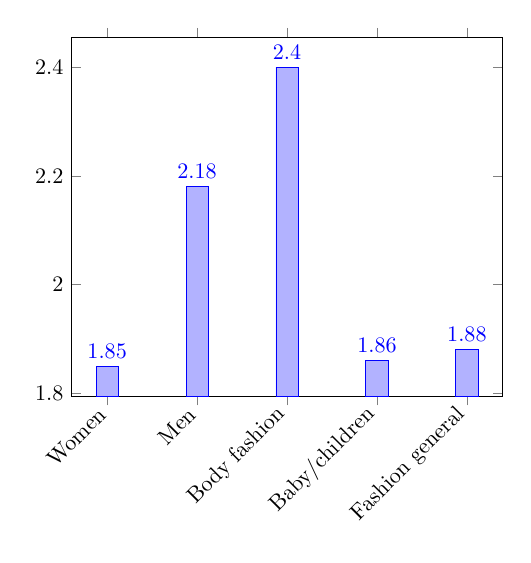
\begin{tikzpicture}[scale=0.8]
      \begin{axis}[
        ybar,
        symbolic x coords={Women, Men, Body fashion, Baby/children, Fashion general},
        x tick label style={rotate=45, anchor=east},
      ]
      \addplot +[nodes near coords] coordinates {
        (Women, 1.85)
        (Men, 2.18)
        (Body fashion, 2.40)
        (Baby/children, 1.86)
        (Fashion general, 1.88)
      };
      \end{axis}
    \end{tikzpicture}
    \caption{Conversion rate in various fashion segments}
\end{figure}

\marginpar{TODO: Conversion rate in SoBazaar?}
This figure is taken from~\cite{Jorij2012} and shows the conversion rate for
various segments in the fashion domain. The conversion rate is the portion of
users who visits a website, and reaches the target (makes a conversion) set
by the site. For most e-commerce application, SoBazaar included, a conversion
is counted when a purchase is made. The conversion rate $r$ can easily be
calulcated by $r = \frac{|Conversions|}{|Total visits|}$~\ref{nielsen2013}.
We can see that womens has the lowest conversion rate among the different
segments, indicating that there is a strong preference based shopping
tendency and that many users are \textit{browsing} and searching for the
right product. This hypthesis is strengthed by looking at the general
conversion rate in the e-commerce industry, which lies at 3\%. The potential
of a personalized recommender could in other words make browsing easier and
hence increase the conversion rate.

\begin{figure}[H]
  \begin{tabular}{cc}
    \resizebox{0.43\linewidth}{!}{
      \begin{tikzpicture}
        \pie[text=legend, rotate=60]{
          34.30/Women,
          13.43/Men,
          17.91/Generalist,
          11.94/Body,
          4.47/Shoes,
          2.98/Jeans,
          14.97/Other
        }
      \end{tikzpicture}
    }
    \resizebox{0.49\linewidth}{!}{
      \begin{tikzpicture}
        \pie[text=legend, rotate=60]{
          15/Direct,
          23/Paid,
          30/Organic,
          5/CPS,
          9/CPC,
          8/Viral or social,
          10/E-mail newsletter
        }
      \end{tikzpicture}
    }
  \end{tabular}
  \caption{Distribution of target groups and traffic sources in the fashion
  domain}
\end{figure}

Both figures are taken from~\cite{Jorij2012}, basing its results from a study
with 70 participating fashion companies with the goal of doing a complete
benchmark of the industry. In the leftmost figure we see how the different
e-commerce fashion retailers focuses their products. We observe that a large
majority of e-commerce fashion companies are targeting women - as is
SoBazaar.  Underlining the comptetative market and the need to stand out to
the customer, by e.g. having personalized recommendations.

In the rightmost figure it is shown from where the customers originate in
online retails stores. The \textit{Paid} and \textit{Organic} are synonymous
with a user entering the site via. research or ads in the search engine, and
stands for 53\% of the traffic in e-commerce fashion - highlihting the
importance of a good reputation and digital profile. Direct traffic is as low
as 15\%, compared to the e-commerce industry in general where the same number
is 22.3\% \cite{Jorij2012}. This is explained by non-fashion products often
being offered in multiple stores and the users are thus browsing multiple
sites to find the best offer. Lastly we note that the viral/social segment is
rather small at 8\%, but compared to the e-commerce industry in general at
4\%. Hence we conclude that although a small of users interacts with fashion
companies by social media, it is a more important segment in this industry
compared to e-commerce in general.

\subsection{SoBazaar, the e-commerce application}
  As briefly mentioned in the introduction chapter~\ref{sec:motivation} SoBazaar is a fashion e-commerce application for web and hand held devices.
  The application is developed by Telenor and aggregates fashion products from various brands and stores, mainly fashion related.
  Users of the application can choose to log in with their social media account on Facebook~\footnote{Facebook is an online social media service with around 1.28 billion monthly active users~\cite{facebook}} to store and share their fashion findings in the application.
  This allows the user to have one entry point to get the latest updates on fashion, and see what the user's social network is up in regards to fashion.
  When the user finds an item especially interesting and is interested in purchasing the item, the user is redirected to the store from which the product originated.

  The fact that SoBazaar utilizes Facebook and a large set of fashion stores lets the users of the application gather at one place to find users with similar taste in fashion.
  As seen from~\ref{subsec:theory} one important aspect in fashion is the feeling of belonging, which is made easy through the utilization of Facebook.

\subsection{Competitors to SoBazaar}
  \label{subsec:competitors}

	\marginpar{TODO: Extend with Asos}
	\marginpar{TODO: Extend with Kwoller}
	\marginpar{TODO: Extend with Mallzee}
	\marginpar{TODO: Mention that many new apps have popped up recently, attempting to do the same as SoBazaar}

    As seen from~\ref{subsubs:fashionInEcom} SoBazaar is not the only e-commerce application for fashion, and has therefore some competitors.
    SoBazaar is built up of a collection of e-commerce store front applications and social interactions, but SoBazaar is not the first of its kind.
    There is a set of other similar applications providing the user with similar possibilities as SoBazaar.
    This section will be used to explore some of these systems, and look into their strengths and weaknesses regarding item recommendation for the user.

\subsubsection{Myntra} % (fold)
\label{par:myntra}
    "Myntra.com is a one stop shop for all your fashion and lifestyle needs" - about Myntra~\cite{myntra}.

    Myntra is one of India's largest e-commerce stores for fashion and aims to  provide a hassle free shopping experience for the user.
    They aim to bring the newest and most in-season fashion products available to the user trough the web store front.
    The brand base of Myntra consists of 500 leading brands from both inside and outside India.

    The web page uses a set of recommendation approaches to inform the user of what they might like, and to increase the user's awareness of different kinds of items. Such as, similar item and most popular.

    \begin{figure}[H]
        \centering
        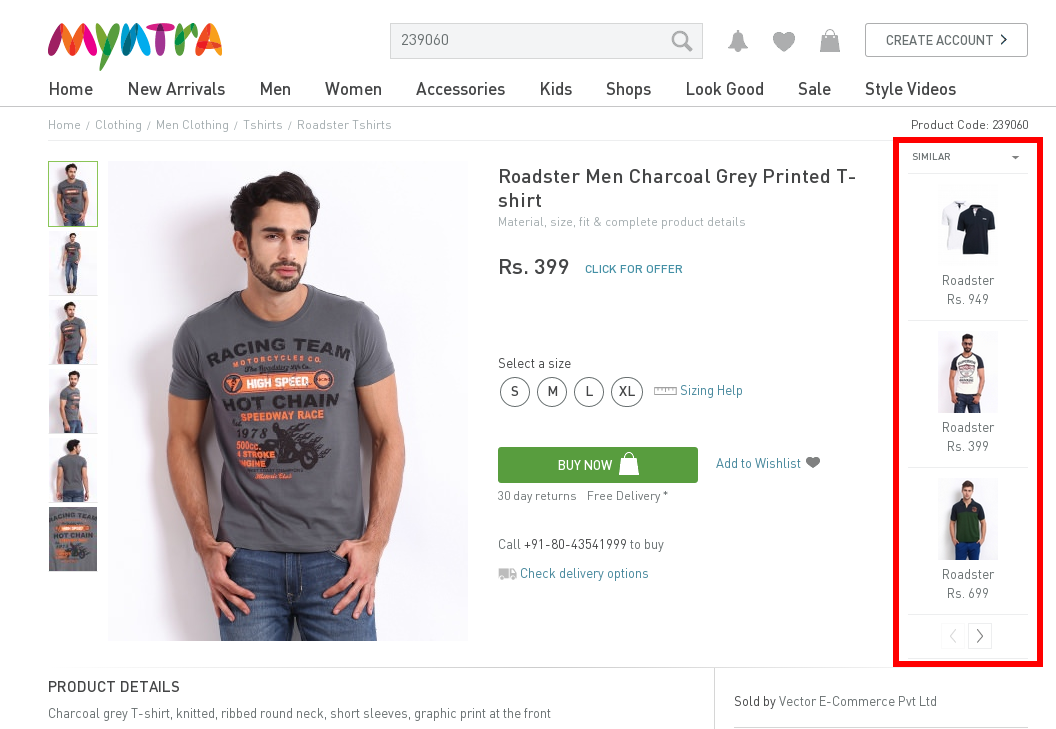
\includegraphics[width=5in]{image/myntiaSimilarExample.png}
        \caption[Example of Myntra's "similar item" approach]{In this figure we can see in red how Myntra is suggesting items which are similar to the item the user is currently looking at}
        \label{figure:myntiaSimilarEx}
    \end{figure}

    \begin{table}[H]
        \centering
        \begin{tabularx}{\linewidth}{>{\parskip1ex}X@{\kern4\tabcolsep}>{\parskip1ex}X}
            \toprule
            \hfil\bfseries Strengths
            &
            \hfil\bfseries Weaknesses
            \\\cmidrule(r{3\tabcolsep}){1-1}\cmidrule(l{-\tabcolsep}){2-2}
            %Strengths
	        Suggest similar items connected to the currently viewed \par
            Popular list for the different brands and stores \par
            Ability to add item to a "want list"\par
            &
            %Weaknesses
            No personalized recommendations \par
            \\\bottomrule
        \end{tabularx}
        \caption[Recommendation related strengths and weaknesses of Myntra~\cite{myntra}]{This table is the list of the recommendation related strengths and weaknesses of the e-commerce fashion web site Myntra~\cite{myntra}}
        \label{table:ecommerceMyntra}
    \end{table}
% paragraph myntra (end)

\subsubsection{Lyst} % (fold)
\label{par:lyst}
    "Lyst.com is a fashion shopping site that gives you your own shopping experience, so you can discover more of the fashion you love" - About Lyst~\cite{lyst}.

    Lyst offers items from thousands of the leading brands and stores of the world.

    The site allows the user to follow different stores or brands to receive the latest items they have to offer.
    The user is given a personalized "stylefeed", which displays items from the different brands or stores the user is following.
    It is also possible for the user to add items to the their profile.

    On first login the user is presented with a set of brands and store the user can like or dislike, to get the "stylefeed" started.
    On access of an item, the user is presented with related items, and the ability to add the item to a collection.
    When the user wants to buy an item, the site will redirect the user to the store selling the item.

    \begin{table}[H]
    	\centering
        \begin{tabularx}{\linewidth}{>{\parskip1ex}X@{\kern4\tabcolsep}>{\parskip1ex}X}
        \toprule
        	\hfil\bfseries Strengths
            &
            \hfil\bfseries Weaknesses
            \\\cmidrule(r{3\tabcolsep}){1-1}\cmidrule(l{-\tabcolsep}){2-2}
                    Can follow brands and stores \par
                    Connected with facebook \par
                    Ability to add item to a "want list" \par
                    "Stylfeed" based the user's follow list \par
                    Show related items \par
                    &
                    Limited personalized recommendations \par
                    \\\bottomrule
                \end{tabularx}
        \caption[Recommendation related strengths and weaknesses of Lyst~\cite{lyst}]{This table is the list of the recommendation related strengths and weaknesses of e-commerce fashion web site Lyst~\cite{lyst}}
        \label{table:ecommenreceLyst}
    \end{table}
% paragraph lyst (end)

\subsubsection{Farfetch} % (fold)
\label{par:farfetch}
    "farfetch.com forms the hub of a global fashion community that unites independent boutiques around the world with fashion lovers" - About Farfetch~\cite{Farfetch}

    Farfetch is a collection of over 1000 boutiques from all over the world gathered on one web page.
    The user can shop directly on the page, and get the item delivered to the doorstep with only one checkout process.

    When browsing an item the user is presented with a set of recommendations related to the current item, and previous browsing history.
    The item can be added to a "want list" or to the shopping chart.
    \begin{figure}[H]
        \centering
        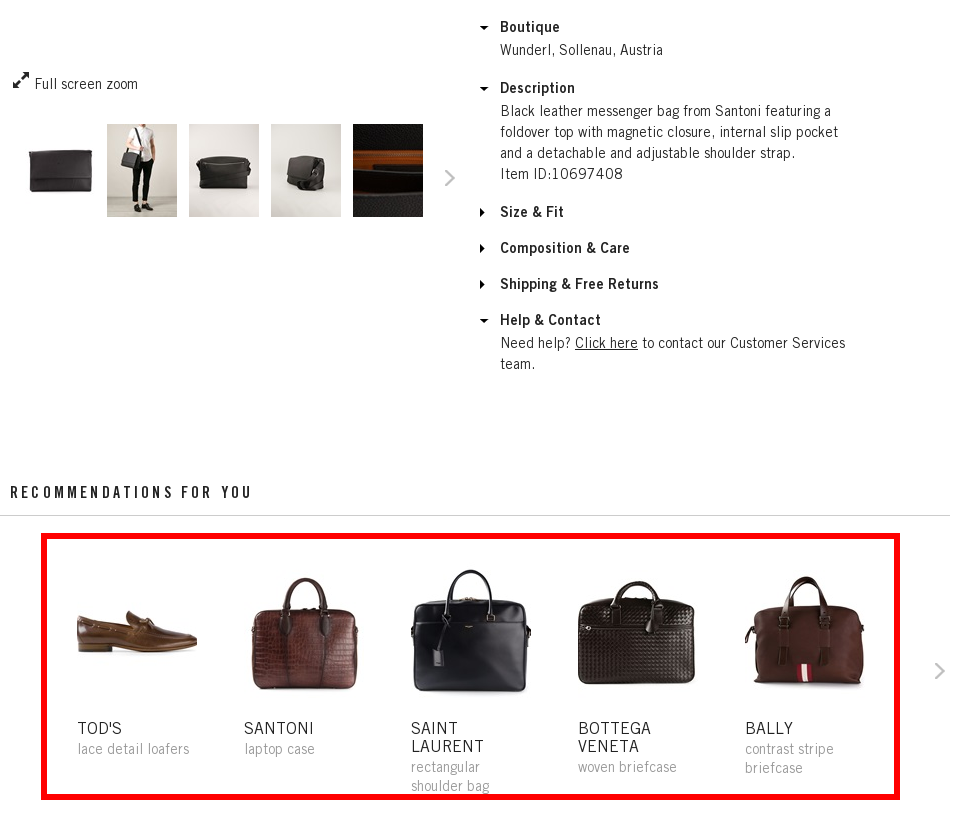
\includegraphics[width=5in]{image/farfetchedRecommendationExample.png}
        \caption[Example of Farfetch's recommendations]{In this figure we can see in red how Farfetch is recommending items which might be of interest to the user. As we can see the first item is a shoe, which was the last item accessed by the user, the next four items are related to the currently viewed item}
        \label{figure:farfetchedRecommendationExample}
    \end{figure}
    \begin{table}[H]
        \centering
        \begin{tabularx}{\linewidth}{>{\parskip1ex}X@{\kern4\tabcolsep}>{\parskip1ex}X}
        	\toprule
        	\hfil\bfseries Strengths
        	&
        	\hfil\bfseries Weaknesses
        		\\\cmidrule(r{3\tabcolsep}){1-1}\cmidrule(l{-\tabcolsep}){2-2}
        		%Strengths
                Ability to add item to a "want list" \par
                A feed with the most popular items \par
                A feed with new items \par
                A list of recommendations for the user \par
            	&
            	%Weaknesses
                No option to follow other users \par
             \\\bottomrule
        \end{tabularx}
        \caption[Recommendation related strengths and weaknesses of Farfetch~\cite{Farfetch}]{This table is the list of the recommendation related strengths and weaknesses of e-commerce fashion web site Farfetch~\cite{Farfetch}}
        \label{table:ecommenreceFarfetch}
    \end{table}
% paragraph farfetch (end)

\subsubsection{MyHabit} % (fold)
\label{par:myhabit}
    "MyHabit is a private fashion sale site offering up to 60% off hand-picked selections from designer and boutique brands." - About MyHabit~\cite{MyHabit}

    MyHabit was founded by Amazon in response to the desire from the users of Amazon to shop fashion in an easy manner.

    The site displays a feed.
    This feed is fed by a team from MyHabit, and is constantly updating with new sales and new products.
    The items put into the feed are handpicked.

    When browsing items on MyHabit, other similar items are suggested to the user.
    \begin{table}[H]
                    \centering
                    \begin{tabularx}{\linewidth}{>{\parskip1ex}X@{\kern4\tabcolsep}>{\parskip1ex}X}
                    \toprule
                    \hfil\bfseries Strengths
                    &
                    \hfil\bfseries Weaknesses
                    \\\cmidrule(r{3\tabcolsep}){1-1}\cmidrule(l{-\tabcolsep}){2-2}
                Shop on site \par
                Similar items \par
             &
                No personalized recommendations \par
            \\ \bottomrule
        \end{tabularx}
        \caption[Recommendation related strengths and weaknesses of MyHabit~\cite{MyHabit}]{This table is the list of the recommendation related strengths and weaknesses of e-commerce fashion web site MyHabit~\cite{MyHabit}}
        \label{table:ecommenreceMyHabit}
    \end{table}
% paragraph myhabit (end)

\subsubsection{Competitors Recommendation Overview} % (fold)
\label{par:competitors_recommendation_overview}
    In table~\ref{table:ecommerceCommpetiros} we see that there is a very low count of fashion related e-commerce applications, which actually produces personalized recommendations for their users.

    Most of applications are taking a simpler approach when making recommendations for the user, like most popular or similar items.
    There is no obvious relation between recommendations and that the site has a form of "want list", but the system which allows the users to follow each other are usually not in-application-purchase-applications.

    There where no indications of the "want list" being used directly to some personalized recommendations and neither was it any indication that the "follow list" of other users helped produce any personalized recommendations, other than recommending items from the followed user's feed.
    The "follow list" was also in some cases used to suggest other users to follow.
    The "want list" was primarily there so that the user could go back to a liked item, and maybe interact with it later.
    \begin{table}[H]
        \centering
        \begin{tabular}{l l l l l l l}
            \toprule
            Competitor &
            \multicolumn{1}{l}{\parbox{1.3cm}{ In App \\ Purchase}} &
            \multicolumn{1}{l}{\parbox{1.0cm}{ Most \\ Popular}} &
            \multicolumn{1}{l}{\parbox{1.0cm}{ Similar \\ Items}} &
            \multicolumn{1}{l}{\parbox{1.0cm}{ Want \\ List}} &
            \multicolumn{1}{l}{\parbox{1.9cm}{ Follow \\ Other Users}} &
            \multicolumn{1}{l}{\parbox{2.6cm}{ Personalized \\ Recommendations}} \\ \midrule

            Myntra  & \cmark & \cmark & \cmark & \cmark & \xmark & \xmark \\
            Flink   & \xmark & \cmark & ?? & \cmark & \cmark & \xmark \\
            Lyst    & \xmark & \cmark & \cmark & \cmark & \cmark & \xmark \\
            Motilo  & \xmark & \cmark & \xmark & \cmark & \cmark & \xmark \\
            Farfetch & \cmark & \cmark & \cmark & \cmark & \xmark & \xmark/\cmark~\tablefootnote{How the recommendations are produced is not mentioned} \\
            ModCloth  & \cmark & \cmark & \cmark & \cmark & \xmark & \xmark \\
            UsTrendy  & \cmark & \cmark & \cmark & \cmark & \xmark & \xmark \\
            Polyvore  & \xmark & \cmark & \cmark & \cmark & \cmark & \xmark \\
            Clothia  & \xmark & \cmark & \cmark & \cmark & \cmark & \xmark \\
            Trendabl  & \cmark & \cmark & \cmark & \cmark & \cmark & \xmark \\
            Zalando  & \cmark & \cmark & \cmark & \cmark & \xmark & \xmark \\
            Ellos  & \cmark & \cmark & \cmark & \cmark & \xmark & \xmark \\
            LookBook  & \xmark & \cmark & \cmark & \cmark & \cmark & \xmark \\
            Fahsiolista  & \xmark & \cmark & \xmark & \cmark & \cmark & \xmark \\
            ShopStyle  & \xmark & \xmark & \cmark & \cmark & \xmark & \xmark \\
            MyHabit  & \cmark & \xmark & \cmark & \xmark & \xmark & \xmark \\
            \bottomrule
        \end{tabular}
        \caption{Properties of different e-commerce application}
        \label{table:ecommerceCommpetiros}
    \end{table}
    Show in the table~\ref{table:ecommerceCommpetiros} above is the list of the different properties of some of the different competitors to SoBazaar. The properties are in regards of their recommendation ability, and how they let their user expand their item set
    A more complete list can be found in the appendix~\ref{app:sec:soCompetitors}.

% paragraph competitors_recommendation_overview (end)

% mtodo
% Diskusjon
%   behold 3 resten til appendix
      % utdyp om SoBazaar, hvordan passer de inn
      % Bruk data til å beskrive at det vi driver med er viktig.
%   Hvborfor har vi dette?
%   Dert er få anbefalinger
%   Dollars er et lukurativt market

  % Heri satte utropstegn ved:
  %   Flink
  %   Lyst og
  %   Motilo

\subsection{Fashion Recommender Systems}
    This subsection will look at different methods other fashion related systems have used to recommend fashion related products to the user.

\subsubsection{Photograph based approach}
    Fashion and the products it regards are highly dependent on visuals.  A fashion
    product would not be very interesting if no one saw it.  An approach to use the
    importance of how the product looks regarding recommending is to utilize images
    of the product.  Fashion Coordinates Recommender System Using Photographs from
    Fashion Magazines~\cite{Iwata:2011} is a system doing this.  They teach their
    system by using fashion magazines with full body images.  They segment the
    image into two parts, top and bottom.  From this the system learns which top
    matches to which bottom and collects visual features of the products.  From
    this the system can recommend other tops to go with a selected bottom, or other
    way around.  The proposed system scored better\footnote{Accuracy of 50\% on the
    top 5 suggested items, whereas naive and random managed 18\% and under 5\%
    respectively} than both a more naive approach and a random selection.  Runtime
    was at 0.04 seconds per recommendation.

\subsubsection{Hot-or-not}
    A recommender system called SuitUp~\cite{SuitUp} did a survey on some of their potential users.
    One interesting finding was that many of the users enjoyed the Hot-or-Not feature of the system.
    This feature gives the user a set of items and the option to either like or dislike.
    This did not only make the participants in the survey more engaged in the system, but also produced ratings, both negative and positive, for the system.
    For cold-start users and in a cold-start system this extra information and ratings make it much easier to make recommendations for the users.

\subsubsection{Scenario-Oriented Recommendation}
    Shen et al.~\cite{Shen:2007:AIG:1216295.1216368} proposed a recommender system which produce recommendations not only based on the metadata of the products, but also on user written input.
    Knowledge used to handle the user input, is derived from Open Mind Common Sense~\cite{Singh02openmind}.

    The user uploads his or her clothes and adds brand (e.g.Nike), type (e.g.jeans), material and a description about the item (e.g."I put these on when I get home").
    The systems makes recommendations based on the scenario the user is needing help to find suiting clothes to wear.
    The typical use case of the system is when a user is unsure about what to wear under different circumstances, but knows something about the scenario or occasion the clothes will be worn in.
    For instance: "I am going to the beach".
    It is also possible to interact with other users and the system relates similar users.

    The different describing fields about the items are given a six-tuple style value.
    The six tuples are: luxurious, formal, funky, elegant, trendy and sporty, where each is given a value from 0 to 10 based on how much the describing field of the items is the current tuple.
    The different describing fields are given a default value, which can be changed by the user if that this necessary. But it seems like this has to be done for all brands, material and type manually to initialize the system.

    This is an interesting approach to fashion and clothes recommendations but the need for user scenario input and a six-tuple description of the different describing fields, might not be desirable for the user or the system administrator in the long run.

    Yu-Chu et al.~\cite{Yu-Chu:2012:PCS:2376365.2376961} and Ying et al.~\cite{Ying2011} are other similar systems. Ying et al.~\cite{Ying2011} made a recommender based on the a similar concept, namely, what to wear in different situations.
    The system recommends two sets of top-to-toe clothing based on the current season, the occasion and the items the user has uploaded.
    The uploaded items must be given a set of descriptions, including the occasion to use the item.

    To recommend, the system uses the user profile of the user, which describes the interests of the user and the information given by the user about the different items in his or hers wardrobe.

\subsubsection{Photograph Recommendation Integrated with Occasion} % (fold)
\label{par:photograph_recommendation_integrated_with_occasion}
    Liu et al.~\cite{Liu:2012:HMC:2393347.2393433} combined the two approaches from Iwata et al.~\cite{Iwata:2011} and Ying et al.~\cite{Ying2011} and Shen et al.~\cite{Shen:2007:AIG:1216295.1216368} and suggested a system which recommend clothes both based on the photographies and the occasion the clothes are to be worn.

    They do this by incorporating fashion rules like, what can you wear to which occasion, and what can you wear as a complete set to different occasions.
    The recommender learn the clothing recommendations through a latent support vector machine framework.
    They use this framework to match four potential functions: visual features vs. attribute, visual features vs. occasion, attributes vs. occasion and attribute vs. attribute.
    These are used together in a scoring function for clothing recommendation.

    Their system preformed better than the baselines, but was highly dependent on the human detection accuracy, since the learner was learning from fashion photographs.
% paragraph photograph_recommendation_integrated_with_occasion (end)

% !TEX root = ../../report.tex

\section{Session Based Approach}
    Different ways of personalizing recommendations have been explored earlier in this chapter, such as: collaborative filtering and content based filtering.
    A common issue with these types recommendations is sparsity in the data, which can lead to poor recommendations.
    Through utilizing usage pattern of the user and producing sessions, some of the sparsity gaps can be filled.
    The patterns can help to understand the pre-purchase patterns, products they see and what they buy.
    This information can also produce interesting relationships between products.
    With this the user preferences can be gathered and be used to reduce the search space when recommending product for the user.

% \subsection{E-commerce}
%     About sessions

\subsection{Mining}
    How to gather information on the user.
    The data mining can be split into two main steps~\cite{Cho2002329}:
    \begin{itemize}
        \item \emph{Data Preparation} - In the data preparation step the sessions are built. They are built based on the usage during a single visit to the application, web page or system the user is accessing. It is the sequence of events produced by the user actions during the visit.
        \item \emph{Pattern Discovery} - In the pattern discovery step the system must use the sessions gathered in the previous step to discover association rules, sequential patterns, usage clusters, page clusters, user classification or any other pattern discovery method.
    \end{itemize}

    \subsubsection{Data Preparation} % (fold)
        \label{par:Data_Preparation}
        When a user accesses an application or web page, the system can store the footprints of the user.
        Within these footprints the system can embed information as browser used by user, location of the user, event triggered by user and time stamp.
        This bundle of information is called an event, a the set of event produced by the user during on application or web page visit, is called a session.

    \subsubsection{Pattern Discovery} % (fold)
        \label{par:pattern_discovery}
        \paragraph{Association Rules} % (fold)
            \label{subp:association_rules}
            The association rule describes how item X and Y are coupled, this coupling is the percentage of transactions that contain both item X and item Y.

            One simple way of discovering this association is through the aprior algorithm~\cite{Agrawal:1994:FAM:645920.672836}.

            With this set of rules for the items, item taxonomies can be used to infer knowledge regarding the items.
            For instance; sessions when buying blue skirts often include buying of red shoes.
        % easy example: http://nikhilvithlani.blogspot.no/2012/03/apriori-algorithm-for-data-mining-made.html
        \paragraph{Sequential Patterns} % (fold)
        \label{subp:sequential_patterns}
            The sequential patterns can be used to build Markov models to predict the next step the user will take based on the sequential pattern of the events from the sessions~\cite{Deshpande:2004:SMM:990301.990304}.

            An issue with using the Markov model is that if first-order is being used, the accuracy can be faulty, since the model will not be looking far enough behind.
            Handling this with an higher-order model might solve the inaccuracy due to too low order, but might cause an issue with high state space complexity, and might also reduce coverage.
            Which can be handled through training a set of K different Markov models, with K different orders, All-$K^{th}$-Order Markov model, but the space complexity issue will still be present.

            The Markov model predicts future actions through looking at past actions.
            So for first-order, the model looks at the last event performed to predict the next event of the user.
            The higher the order, the further back the model is looking in the event set and will produce a more complicated model, the higher the order.
            This can be handled through the usage of a selective Markov model~\cite{Deshpande:2004:SMM:990301.990304}

            One issue with the Markov model is that a user will not get predicted new items if the sessions used to predict future actions are only based on the own users sessions.
            One way of making use of the patterns and producing new recommendations is trough matching sequential patterns from users with one-another. \marginpar{something not right}


        \paragraph{Usage Clusters} % (fold)
        \label{subp:usage_clusters}
            The usage clusters are usually built up from the different features of the events in the session.
            Where the features are collected an used to model the user.

            \begin{table}[H]
                \centering
                \begin{tabular}{l|l}
                    \emph{Event features} & \emph{Description} \\ \hline
                    Amount of purchases & - \\ \hline
                    Amount of viewsts & - \\ \hline
                    Amount of wants & - \\ \hline
                    Time on items under the different conditions mentioned above & -\\ \hline
                    Overall average time on items & - \\ \hline
                    Click to buy rate & - \\ \hline
                    Search query~\cite{Zhang:2006:MSE:1135777.1136004} & - \\ \hline
                    What was done before a specific action & - \\ \hline
                    What was done before a specific action & - \\
                \end{tabular}
                \caption[Event Features]{Set of event features used for finding usage clusters and model the users behavior}
                \label{table:uasageCluster}
            \end{table}

        \paragraph{Page Clusters} % (fold)
        \label{subp:page_clusters}
            Page clustering will help the system to understand which pages belong together.
            For instance when searching for Harry Potter, the user might have interest in knowing more about the author J.K. Rowling, and the system might benefit from clustering queries of here with Harry Potter~\cite{Zhang:2006:MSE:1135777.1136004}.

        % \paragraph{User Classification} % (fold)
        % \label{subp:user_classification}

\subsubsection{Session Examples} % (fold)
    \label{par:session_examples}
    \marginpar{Show three common user session patterns (average purchase time, want time and view time)}
    A user session of a user randomly chosen user.
    \begin{lstlisting}
        { "event_id" : "app_started", "product_id" : "NULL", "ts" : NumberLong("1382689141084") }
        { "event_id" : "storefront_clicked", "product_id" : "NULL", "ts" : NumberLong("1382689144152") }
        { "event_id" : "storefront_clicked", "product_id" : "NULL", "ts" : NumberLong("1382689172026") }
        { "event_id" : "storefront_clicked", "product_id" : "NULL", "ts" : NumberLong("1382689179152") }
        { "event_id" : "product_detail_clicked", "product_id" : 2028030, "ts" : NumberLong("1382689192035") }
        { "event_id" : "product_purchase_intended", "product_id" : 2028030, "ts" : NumberLong("1382689197749") }
        { "event_id" : "product_detail_clicked", "product_id" : 2038024, "ts" : NumberLong("1382689263384") }
        { "event_id" : "storefront_clicked", "product_id" : "NULL", "ts" : NumberLong("1382689284693") }
        { "event_id" : "storefront_clicked", "product_id" : "NULL", "ts" : NumberLong("1382689297864") }
        { "event_id" : "storefront_clicked", "product_id" : "NULL", "ts" : NumberLong("1382689322201") }
        { "event_id" : "storefront_clicked", "product_id" : "NULL", "ts" : NumberLong("1382689326804") }
        { "event_id" : "storefront_clicked", "product_id" : "NULL", "ts" : NumberLong("1382689352841") }
        { "event_id" : "product_detail_clicked", "product_id" : 2028032, "ts" : NumberLong("1382689357563") }
        { "event_id" : "product_detail_clicked", "product_id" : 2038025, "ts" : NumberLong("1382689363957") }
    \end{lstlisting}

    purchase time: 14068.69687
    want time: 17859.1539

% ~\cite{Kelly:2003:IFI:959258.959260}


\subsubsection{Multi-Armed Bandit} % (fold)
    \label{par:multi_armed_bandit}
    \marginpar{might be interesting as an most popular approach, suggest the most popular at any one time, belongs with most popular approach}

\subsubsection{Analyzing}
    Analyzing the model of the user

\subsection{Recommending}
    Using the model to help personalizing the recommendation for the user

\subsection{Limitations}
    What are the limitations of a session based approach to recommendations.


% % !TEX root = ../../report.tex
\section{One-Class Collaborative Filtering}

% todo - hva vil vi med denne sekjsonen?

\subsection{About}
    There are many applications where the feedback from a user is in binary form.
    Take for instance a item purchase page without explicit feedback.  The only
    feedback from a user might only be if an item has been purchased or not, the
    data consists only of binary data.  Other cases can include page visitation or
    webpage bookmarking.  The fallout of this is that the data collected from the
    user is usually really sparse.  And one issue which arises from the binary
    feedback is the lack of known negative feedback.  Does the fact that a user
    visited a web page, but not another indicate that the user dislikes the
    unvisited page, or simply that the user oversaw it?  The negative feedback and
    the missing feedback are mixed together in the bigger part of the dataset.
    Which makes it difficult to identify what is what.  Recommendations, through
    finding the missing positives, done on these types of data is usually thought
    of as one-class collaborative filtering (OCCF).  OCCF can be viewed as an
    extreme case of class imbalance, in which the balance is only distributed over
    one class. \marginpar{checkout Extreme re-balancing for svms: a case study
    maybe}

\subsubsection{Common OCCF Scenarios}
    Some of the most common scenarios where the OCCF problems occurs are:
    Bookmarking, click history, product purchase, "like" and news reader.  The data
    produced from user feedback from all these scenarios can be on the binary form.

\subsection{Different approaches}
    To handle the problem with the sparse data mixed with the ambiguous missing
    data, several strategies has been proposed.

\subsubsection{Negative ratings}
    Since one of the main issues are with the missing data, a natural approach
    would be to gather more.  One way of doing so is by asking the user to rate
    more items.  This can be done through forcing the user to rate a set of
    predetermined items and/or produce negative ratings to uninteresting items.
    The issue with this approach is that putting the rating burden onto the user
    has shown to produce negative user
    experience~\cite{Kelly:2003:IFI:959258.959260}

\subsubsection{All missing as negative (AMAN)}
    One naive approach is to view all the missing values as negative values.
    Thereby saying all web pages ignored by the user are unwanted pages.  One issue
    with this approach is that it will render examples which are positive, but
    unknown, as false negatives.

\subsubsection{All missing as unknown (AMAU)}
    Another naive approach is to go in the opposite direction.  Viewing all missing
    values as unknown, thereby only utilizing the known values when recommending,
    the predictions on the unknown values will only be positive.  The data in an
    OCCF problem is also usually very sparse, therefore using only the positive
    examples will in many cases lead to an incomplete view of the data, and quality
    reduced recommendations.

\subsubsection{Weighted low-rank approximation}
    \cite{pan2008} \cite{Nati03weightedlow-rank}
    The idea behind this approach is to distribute different weights to the unknown
    values.

    More specifically, given two matrices, one rating matrix $R = SxC$, where $S$
    is a list of $m$ items, $S = {s_{1},...s_{m}}$ and $C$ is a list of $n$ users,
    $C = {c_{1}, ... c_{n}}$.
    $R$ has a corresponding weight matrix $W$, where $S$ is a list of $m$ items, $S
    = {s_{1},...s_{m}}$ and $CWz$ is a list of $n$ users, $C = {c_{1}, ... c_{n}}$.
    The values in $R$ are either 0 or 1, and the values in $W$ are between 0 and 1.
    With these two matrices, weighted low-rank approximation is meant to find a low
    rank matrix $X$.  Done through the Frobenius norm, which is minimizing the sum
    squared differences to the target matrix~\cite{frobeniusNorm}.  Other
    approaches to the weighting issue has been taken, such as low-density
    non-negative matrix factorization~\cite{Sindhwani:2010:OMC:1933307.1934641}.

    \begin{equation}
        J(X) = \sum_{mn} W_{mn}(R_{mn} - X_{mn})^2
        \label{equation:frobenius}
    \end{equation}

    Equation~\ref{equation:frobenius} can be optimized and solved efficiently
    though the use of wighted ALS~\citep{Koren2009}.  The positive values are set
    to 1 in the $R$ matrix, and the negative set to 0.
    Since the positive values have a high certainty of being correct, the
    corresponding wight from the matrix $W$ is set to 1.  For the unknown values
    the corresponding weight is set after a weighting schema.  Where the weight is
    lowered for more certain negatives.  This weight is between 0 and 1.  Another
    approach to handling the

    \begin{table}[H]
        \centering
        \begin{tabular}{l|l|l}
          \emph{Schemes}      & \emph{Pos Examples} & \emph{Neg Examples} \\ \hline
          Uniform               & $W_{mn} = 1$ & $W_{mn} = [0,1]$ \\ \hline
          User-Oriented         & $W_{mn} = 1$ & $W_{mn} = UO(\sum_{n} R_{mn})$ \\ \hline
          Item-Oriented         & $W_{mn} = 1$ & $W_{mn} = IO(m - \sum_{n} R_{mn})$ \\ \hline
          User-Item interaction & $W_{mn} = 1$ & $W_{mn} = E(I)$  \\ \hline
          User-Item similarity & $W_{mn} = 1$ & $W_{mn} = S(I,U)$  \\
        \end{tabular}
        \caption[Weighting Schemes]{Different ways of weighting ratings suggested by \cite{pan2008}}
        \label{table:WeightingSchemes}
    \end{table}

    Different weighting schemes are show in~\ref{table:WeightingSchemes}.

    The uniform approach considers all negative examples in the same way, and
    thereby assigns the same weight to all the negative examples.  The
    user-oriented scheme assumes that if a user has more ratings, the negative
    examples can be weighted to be more negative.  The item-oriented assumes that
    if there are more positive example for an item, the missing data is negative
    with a lower probability.  The last scheme, the user-item interaction
    approach, takes into consideration the events on the item to be considered.
    For instance clicks and views.

    \paragraph{User-Item similarity} % (fold)
        \label{subp:user_item_similarity}
        In the user-item similarity approach, the items content of the items and from the users are extracted based on the examples in the data where the positive examples are set to 1.
        From this there is built models for the users and the item.
        The similarity between the user and the item is then used to give the negative examples a weight~\cite{yuan2013}.

\subsubsection{Negative example sampling~\cite{pan2008}}
    In many cases the missing values are in fact negative values.  This approach
    will i most cases lead to a large rating matrix, and therefore high
    computational costs.  Therefore, instead of using all the ratings in the
    ratings matrix $R$, only all the actual positive values are selected.  This is
    combined with a subset of the presumed negative values.  This subset is based
    on a sampling probability matrix $P$.

    There are different sampling schemes.
    Using the same schemes as from weighted low rank approximation.

\subsubsection{Group Bayesian personalized ranking (GBPR)~\cite{Pan:2013:GGP:2540128.2540516}}
    Utilizing rich user interaction.  Group preference is the preference score of a
    group of user on an item.  GBPR assumes that the group preference is stronger
    than the observed user preference.

\subsubsection{Incorporating Rich User Information~\cite{deLace2010,Li2013}}
    When dealing with implicit feedback extra information is usually available
    regarding the user and item.  For instance search query, click history, view
    time and purchase history.  Two ways of incorporating this information has been
    proposed in~\cite{deLace2010}.  One is through linearly combining cores from
    the different sources, and the other is through embedding user information into
    collaborative filtering.

% \subsubsection{Em algorithms to predict negative examples}
    % \cite{Nati03weightedlow-rank}
    % % \todo{check out the approaches}
    % PEBL: positive example based learning for web page classification using SVM
    % Building text classifiers using positive and unlabeled examples
    % Presence-only data and the EM algorithm

    % \subsubsection{Low-density non-negative matrix factorization (ldNMF)}
    % \cite{Sindhwani:2010:OMC:1933307.1934641}
    % arg min
    % J W, H, {y ij } (i,j)∈U =
    % W ≥0,H≥0
    % y ij ∈{0,1},(i,j)∈U
    % λ W
    % 2
    % F
    % + γ H
    % 2
    % F
    % C ij V (X ij , w i T h j )
    % +
    % (i,j)∈L
    % C ij V (y ij , w i T h j )
    % +
    % (i,j)∈U
    % % \todo{make equation}
    % Equation.
    % $R = SxC$ % \todo{0 or 1} is the rating matrix, where $S$ is a list of $m$ items, $S = {s_{1},...s_{m}}$ and $C$ is a list of $n$ users, $C = {c_{1}, ... c_{n}}$.
    % $L$ is the set of positive ratings, while $U$ is the set of unlabeled rating.
    % $W$ and $H$ are the latent factors.
    % $V$ is a loss function (squared loss or generalized KL-divergence).
    % $C$ is the entry specific costs.
    % γ ≥ 0 and $λ$ tradeoff the regularizers againts the fata-fit terms.

\subsection{Discussion}
% todo discuss

% !TEX root = ../../report.tex
\section{Evaluation}
\label{evaluation}

	% What evaluation methodologies exist?
		% Offline Evaluation
		% 	Recommender System Datasets
		%		Explicit vs. Implicit
		% 	Offline Evaluation Measures
		%		Traditional evaluation measures
		%		Cold-start system evaluation
		%		Implicit feedback evaluation measures
		% Online Evaluation


%Some key questions in evaluating recommender systems on testbed data are: what
%to predict, how to grade performance and what baseline to compare with.

In most cases a system designer that wish to employ a recommender system must
choose between a set of candidate approaches. A first step towards selecting an
appropriate algorithm is to decide which properties are the most important for
the application. Recommender systems have a variety of properties such as
accuracy, robustness, scalability, etc. The following section will discuss how
to compare recommender systems based on the set of properties  relevant for the
application and how to evaluate the performance of the system. We have several
different experimental settings which can be used to evaluate recommender systems.
We will focus on two types of experiments:
Offline experiments where the system is evaluated without user interactions and
Online experiments where real users interact with the system. This section will
also cover some of the most frequently used evaluation metrics, a discussion on
the suitedness of different evaluation measures for implicit feedback, and
summary of the methodologies and evaluation measures used to evaluate the
cold-start performance of recommender systems.

Shani et al.\ \cite{Shani2011} lists the following guidelines for general
experimental studies:

\begin{itemize}
	\item Hypothesis: before running an experiment one must form an hypothesis. For
		example, an hypothesis can be that algorithm $A$ better predicts user ratings
		than algorithm $B$. In that case the experiment should test the prediction
		accuracy, and not look at other factors.

	\item Controlling variables: when comparing a few candidate algorithms on a
		certain hypothesis, it is important that all variables that are not tested
		are fixed.

	\item Generalization power: when drawing conclusions from experiments, we may
		wish that our conclusions generalize beyond the immediate context of the
		experiments. When choosing an algorithm for a real application, we may want
		our conclusion to hold on the deployed system, and generalize beyond the
		experimental data set. To increase the probability of generalization of the
		recommender results one must typically experiment with several data sets or
		applications.
\end{itemize}

\subsection{Offline Evaluation}
Offline experiments are performed using pre-collected dataset\(s\) and a protocol
that models the user behavior to estimate recommender performance through
different evaluation measures. Offline experiments are attractive because they
require no interactions with real users, and thus allows multiple  researchers to compare
a wide range of algorithms, using the same data, at a low cost. The downside of offline experiments
is that they can answer a very narrow set of questions, typically questions
about the predictive power of the algorithm, and does not measure other user
factors.

\subsubsection{Datasets for Offline Evaluation}

The main aim of a recommender system is to identify the set of items in a
dataset that might be interesting to a user based on their expressed
preferences. For a fashion recommender this would mean estimating how much a
user might like an item, by e.g.\\ predicting what rating a user might give an
item. In recent years, various test collections for different domains such as
books, music, movies have been made available to the public. These datasets
usually consist of user ratings in the form of $(UserID, ItemID, Rating)$,
but may also include a timestamp.

In recent years more or more datasets have been made available which contains
additional information such as demographic information about the users,
trust-networks, user-assigned tags and etc. Under we have listed a few selected
popular datasets containing additional information:

%TODO - Find more cool dataset

\begin{itemize}

\item MovieLens 100k dataset~\cite{Movielens}: The movielens dataset
	incorporates demographic information about the user in addition the
	traditional rating matrix

\item Epinions dataset~\cite{Epinions}: The Epinions dataset includes a
	trust-network, which specifices who-trust-whom in a social network based on
	customer reviews for the website Epinions.com

\item The Million Song Dataset~\cite{Bertin-Mahieux2011}: The million song
	dataset is a implicit feedback dataset. This data also includes information on the users,
	and audio features and song meta-data.

\item The Book-Crossing Dataset: The bookcrossing dataset consists of both implicit and explicit feedback,
	demographic information about users and some content based information about the books.
\end{itemize}

\paragraph{Explicit-feedback}
The definition of explicit is defined as `stated clearly and in detail, leaving
no room for confusion or doubt'. Explicit feedback are more precise than
implicit feedback, but more difficult to collect since it requires active user
involvement. One serious implication of this is that the amount of feedback
often is scarce since many users opt not to provide any feedback. Explicit
feedback mechanisms allow the users to unequivocally express their ratings on a
scale (usually in the form of a Likert scale (strongly disagree – strongly
agree). Thus explicit feedback is able to capture both negative and positive
feedback, while implicit feedback \emph{only} can be positive. It is worth
noting that explicit feedback tend to concentrate on either side of the rating
scale, as users are more likely to express their preference if they feel
strongly for or against an item~\cite{Jawaheer2010}.

\paragraph{Implicit-feedback}
Unlike explicit feedback, we do not have any direct input from the user
regarding their personal preferences. In particular we do not have any
substantial evidence of which items the user dislikes, such as low ratings.
What we do have is indications of whether a user likes an item trough clicks, wants and purchases. Where wants and purchases can be viewed as a form of explicit rating only counting positively.
Implicit-feedback is more easily collected than explicit-feedback, and usually more abundant.
Types of implicit feedback include purchase history, browsing history,
search patters, or even mouse movements. For example, a user who purchases
many clothes from the same brand probably likes that brand. For a larger
discussion surrounding the differences between implicit and explicit
feedback, see Section~\ref{implicit-feedback}

\subsubsection{Validation Methods}
Validation techniques are motivated by two fundamental problems; model
selection and performance estimation. Almost all pattern recognition techniques
have one or more free parameters, and we want a way to select the
\emph{optimal} parameter\(s\) or model for a given problem. Once we have chosen a
model, we wish to estimate how well it is doing.

\paragraph{The Holdout Method}
When using the holdout method you split the dataset into two groups; a training
set used to train the classifier and a test set used to estimate the error rate
of the trained classifier. The Netflix Prize Competition~\cite{Netflix}
provided a training set consisting of 100,480,507 ratings given by 480,189
users to 17,300 movies. The testset consisted of 2,817,131 items where the
ratings were unknown. The submitted predictions were scored against the true
ratings in terms of root mean squared error (RMSE), and the goal was to
minimize this error.

The holdout method has two basic drawbacks; (1) In problems with sparse
datasets we may not be able to afford the luxury of setting aside a portion of
the dataset for testing, (2) Since it is a single train-and-test experiment,
the holdout estimate can be misleading if we happen to get an `unfortunate'
split.

\paragraph{Cross-Validation}
K-fold Cross-Validation creates a K-fold partition of the dataset. For each of
the $K$ experiments, use $K-1$ folds for training and the remaining one for
testing. By setting $K=2$, this is the same as the holdout method. The estimated
error is found by taking the average error from all the experiments.

Leave-one-out is the degenerate case of K-fold Cross-Validation, where $K$ is
chosen as the total number of examples. For a dataset with $N$ examples we
perform $N$ experiments. For each experiment we use $N-1$ examples for training
and the remaining example for testing. Again, the true error is found by taking
the average error rate from the experiments.

In practice the number of folds often depends on the size of the dataset. For
large datasets, even 3-Fold Cross Validation will be quite accurate, which for
sparse datasets, one may wish to train as many examples as possible. A common
choice is $K$ value between 5 and 10.

\subparagraph{Advantages}
One positive aspect with k-fold cross-validation is that the result is averaged over the $K$ experiments. The strongest argument for using cross-validation is the potential of using the entire training set for testing (albeit not at once), creating the largest possible test set for a fixed training data set.

\subparagraph{Disadvantages}
The main disadvantage with K-fold Cross-Validation is the training algorithm has
to be run $K$ times, and thereby increasing the runtime for producing an
evaluation of the system. If the dataset is large, an increase of $K$ runs could
prove to be disadvantageous.
%TODO - more?

\paragraph{Bootstrapping~\cite{efron1994introduction}}

\marginpar{Helge: Føler at bootstrapping er på et annet nivå enn holdout og cross-validation. Passer det, og passer det her?}
\marginpar{Fix}
Bootstrapping is used to estimate properties of an estimate, such as bias, variance, confidence, intervals and prediction error. This is done trough measuring these properties when sampling from an approximated distribution,
creating an empirical distribution of the observed data.
Since the entire population is unknown it will not be possible to calculate the true error from the sample data.
The idea then is that with this information from sample data it is possible to say something about the population.
Since it will not be possible to perform inference on:

\emph{sample data} $\rightarrow$ \emph{population} this is modeled as:
\emph{re-sample data} $\rightarrow$ \emph{sample data}.
The \emph{re-sample data} is a re-sampling of the sample data.

In practice an example to bootstrapping is when we want to calculate the average height of the population worldwide.
The issue here is that it is not as doable to measure everyone, so a subset of the population is used.
Since the average on this number only will be an estimate of the actual world wide average a sense of error margin must be introduced.
Bootstrapping is then used to reduce the error of margin through re-sampling the sample data a large number of times~\footnote{Numbers vary on sample size, but is often 1 000 to 10 000}, and new averages are calculated.
With these averages a histogram can be produced, which provides an estimate of the distribution of this average.

\begin{figure}[H]
    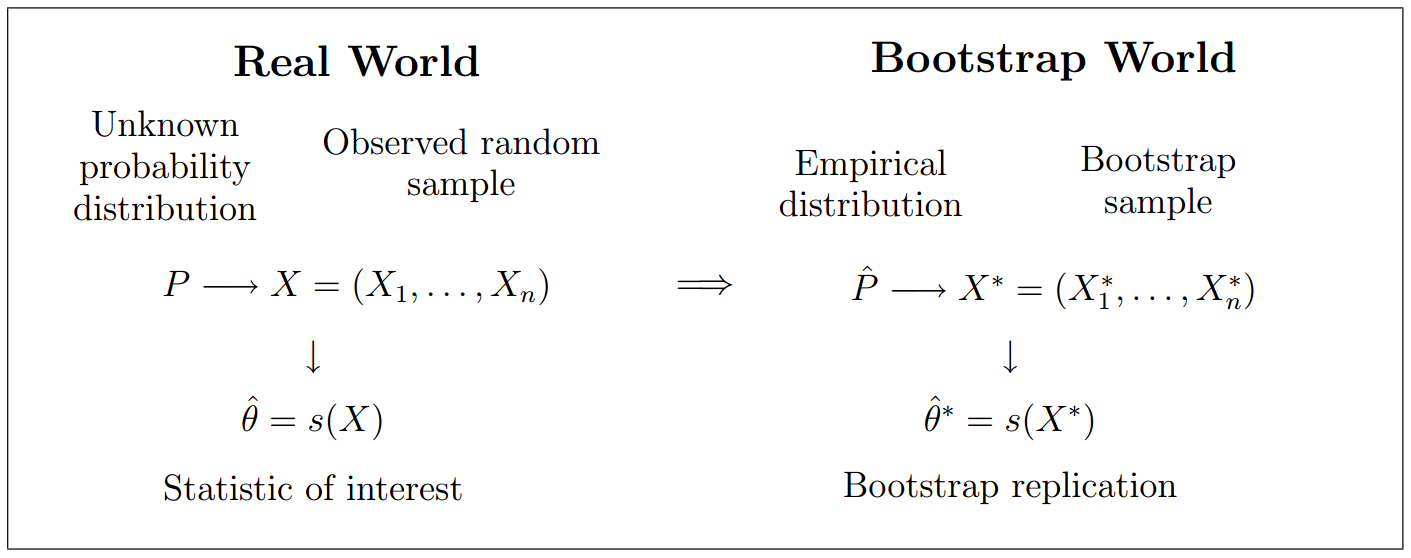
\includegraphics[width=5in]{image/bootstrap.png}
    \centering
    \caption[Bootstrapping principles]{A figure of the principles bootstrapping. Taken from~\cite{Eichler2003}}
    \label{figure:bootstrapping}
\end{figure}

\paragraph{Disadvantages}
	One prominent issue with bootstrapping is that important properties of the actual data might not be caught when undertaking the bootstrapping analysis
	~\footnote{"Bootstrapping" comes from the phrase, "to pull oneself up by one's bootstraps"~\cite{bootstrapSaying1843}}.


\paragraph{Finding the optimal parameter settings}

Finding the optimal parameters for a model is usually a crucial task in engineering approaches to classification and modeling tasks. An automated approach is particularly desirable when the number of parameters is high. In order to work well many algorithms and modeling techniques in computer science rely on a careful choice of their parameters. The usual approach is to select parameters based on some prior experience on the problem at hand with a limited heuristic search of possibly optimal parameters. When such prior knowledge is absent or cannot be directly applied to the technique being used, the optimal parameters have to be found by \emph{blind} search, by e.g. using genetic algorithms or some kind of exhaustive grid-search procedure.

The \emph{de facto} standard way of performing model selection optimization is grid search, which is simply an exhaustive searching through a manually specified subset of the hyperparameter space of a learning algorithm. To \emph{guide} the grid-search one typically uses a performance metric, typically measured by cross-validation on the training set. After evaluating the performance all the pre-specified combinations of parameter settings, the grid search algorithm outputs the setting that achieved the highest score in the validation procedure.

Many of the most popular Machine Learning libraries now come with methods for performing grid search.

\subsubsection{Offline Evaluation Metrics}

When evaluating a recommender system, you wish to estimate a user's
satisfaction for a given recommendation. Traditionally recommender systems have
been evaluated by means of predictive accuracy. However, there is now a widely
agreed that accurate predictions are crucial but insufficient to deploy a good
recommendation engine~\cite{Shani2011, McNee2006}. Some of the properties can
be traded-off, one such example is the trade-off between accuracy and
diversity. It is important to understand and evaluate these trade-offs and
their effect on the overall performance. This subsection will cover the most
popular metrics used for offline evaluation, a discussion of evaluation
measures for implicit feedback, and a summary of the cold-start evaluation
methodologies found in the literature.

\paragraph{Predictive Accuracy Metrics}

Predictive accuracy metrics measure how close the predicted ratings are to the
true user ratings. More formally, the system tries to predict ratings
$\hat{r(c,i)}$ for a test set $T$ of user-item pairs $(c, i)$ for which the
true ratings are known. Traditionally, mean absolute error (MAE) has be used to
evaluate the performance of collaborative-filtering algorithms, but other
measures such as root mean squared error (RMSE) are also commonly used.

\subparagraph{Mean Absolute Error (MAE)}

MAE measures how close the predictions are to the actual outcome.

\begin{equation}
    MAE = \frac{1}{n}\sum_{i=1}^{n}{|\hat{r(c,i)}-r(c,i)|}
    \label{equation:mae}
\end{equation}

$r(c,i)$ is the actual outcome and $\hat{r}(c,i)$ is the predicted value.
As the name suggest, $MAE$ calculates the average absolute error.

\subparagraph{Root Mean Squared Error (RMSE)}

Often used to measure difference between a set of predicted values with a set of actual values.

\begin{equation}
    MSE = \frac{1}{n}\sum_{i=1}^{n}{(\hat{r(c,i)} - r(c,i))^{2}}
    \label{equation:mse}
\end{equation}

\begin{equation}
    RMSE = \sqrt{MSE}
    \label{equation:rmse}
\end{equation}

In $MSE$~\ref{equation:mse} $\hat{r(c,i)}$ is the predicted value and $r(c,i)$ is the actual value.
Both $MAE$ and $MSE$ are used to measure how correct the predictions are compared to the actual values.
$RMSE$ is the square root of $MSE$ and is one of the most used metrics to compare recommender algorithms in collaborative filtering, and was the main metric used in the Netflix price competition to evaluate the performance of the competitors recommender systems. $RMSE$ is always bigger or equal to $MAE$, $RMSE$ penalize an error more than $MAE$.

% \todo{maybe some sweet table of the different algorithms with their eqations and their contributions}
% \begin{table}[H]
%     \centering
%     \begin{tabular}{l|l|l}
%     	% \rowstyle{\bfseries}
%     	Metric	& Equation & About \\ \toprule
%     	MEA 			& \parbox{6cm}{\equationMEA} & safd \\	\hline
%     	RMSE 			& \parbox{6cm}{\equationRMSE} & asdf \\
%     \end{tabular}
%     \label{table:predictiveAccuracyMetrics}
%     \caption [Predictive Accuracy Metrics]{adsf}
% \end{table}



\paragraph{Measuring Usage Prediction}
\label{para:measuring_usage}
% \subsubsection{Decision Based Metrics}
In many applications the recommender system does not predict the user's
preferences of items, but tries to recommend to users items that they may use.
This is often done by giving the user a top-K set of recommendations.
In an offline evaluation of usage prediction, we typically have a dataset
consisting of items each user has used. We then select a test user, hide some
of her selections, and ask the recommender to predict a set of items the user
will use. We then have four possible outcomes for the recommend and hidden
items.

\begin{table}[H]
	\centering
	\begin{tabular}{l l l}
	\toprule
					&	Relevant			&	Not Relevant \\ \midrule
	Recommended		&	True-Positive (TP) 	&	False-Positive (FP)	\\ 
	Not Recommended	&	False-Negative (FN)	&	True-Negative (TN)	\\ 
	\bottomrule
	\end{tabular}
	\label{table:usageprediction}
	\caption[Usage prediction (Confusion Matrix)]{This table is showing the different categories recommended items can end up in.}
\end{table}

\begin{table}[H]
	\centering
	\begin{tabular}{l l}
		\toprule
		True-Positive (TP)	& The recommended item is of interest to the user \\ 
		False-Positive (FP)	& The recommended item is not of interest to the user \\ 
		False-Negative (FN)	& The item is of interest to the user, but is not recommended \\ 
		True-Negative (TN)	& The item is not of interest to the user, but is not recommended \\
		\bottomrule
	\end{tabular}
	\label{table:predictionCategories}
	\caption[Prediction Categories]{}
\end{table}

This model assumes that not relevant items would not have been relevant if they had been
recommended to a user. This assumption may be false, such as when the set of
not relevant items contains some interesting items that the user did not select. For
example, a user may not have relevant an items because she was unaware of its
existence, but after the recommendation exposed that item, the user can decide
to select it. We can count the number of examples that fall into each cell in
the table and compute the Precision, Recall, Fallout and $ROC$.

\subparagraph{Precision}
Precision is the fraction of retrieved items that are relevant.
\begin{equation}
    Precision = \frac{TP}{TP+FP}
    \label{equation:precision}
\end{equation}
Precision takes all recommended items into account, but it can also be evaluated at a given cut-off point, only considering the top $n$ results returned. This measure is called precision at n or P@n.

\subparagraph{Recall}
Recall is the fraction of the items that are relevant to that are successfully recommended.
\begin{equation}
    Recall = \frac{TP}{TP+FN}
    \label{equation:recall}
\end{equation}
Recall can therefore be seen as the probability that a relevant item is retrieved by the recommender.

\subparagraph{Fallout}
Fallout is the amount of retrieved items which is not relevant amongst all the non relevant items (false positive).
\begin{equation}
    Fallout = \frac{FP}{FP+TN}
    \label{equation:fallout}
\end{equation}
Fallout can therefore be looked at as the probability that a non-relevant item is recommended.

\subparagraph{F-measure}
F-measure combines the precision and the recall.
\begin{equation}
    F_\beta = \frac{(1 + \beta^2) * (Precision * Recall)}{(\beta^2 * Precision + Recall)}
    \label{equation:f-measure}
\end{equation}
Based on the value of $\beta$ F-measure will weight precision or recall more. For a $\beta$ over 1 F-measure will emphasize precision over recall, and opposite for $\beta$ between 0 and 1.

\subparagraph{Accuracy}
Accuracy is the amount of correctly recommended items over all the items.
\begin{equation}
    Accuracy = \frac{TP+TN}{TP+TN+FP+FN}
    \label{equation:accuracy}
\end{equation}

\subparagraph{Receiver Operating Characteristics (ROC)}
The $ROC$ is the recall rate ($TPR$) against the fallout rate ($FPR$).
The goal is to maximize the recall while minimizing the fallout.
\begin{equation}
    TPR(T) = \int_T^\infty P_0(T)dT
    \label{equation:tpr}
\end{equation}
\begin{equation}
    FPR(T) = \int_T^\infty P_1(T)dT
    \label{equation:fpr}
\end{equation}
$T$ is a threshold parameter.
The ROC curve is $TPR$ plotted together with $FPR$ at various $T$.

\begin{equation}
    AUROC = \int_\infty^{-\infty} TPR(T)P_0(T)dTdT
    \label{equation:auroc}
\end{equation}
Equation~\ref{equation:auroc} can be used to calculate the area under the curve.
$AUROC$ is the probability that the recommender system will rank positive examples higher than negative examples.
The Area Under is a commonly used evaluation method for binary choice problems. If somebody makes random guesses,
the ROC curve should be a diagonal line stretching from (0,0) to (1,1), as shown by the blue line in Figure \ref{fig:aucroc}, scoring an AUC of 0.5. A perfect model will score an AUC of 1.0. In practice, almost all models will fit somewhere in between.

\begin{figure}[H]
\label{fig:aucroc}
  \centering
    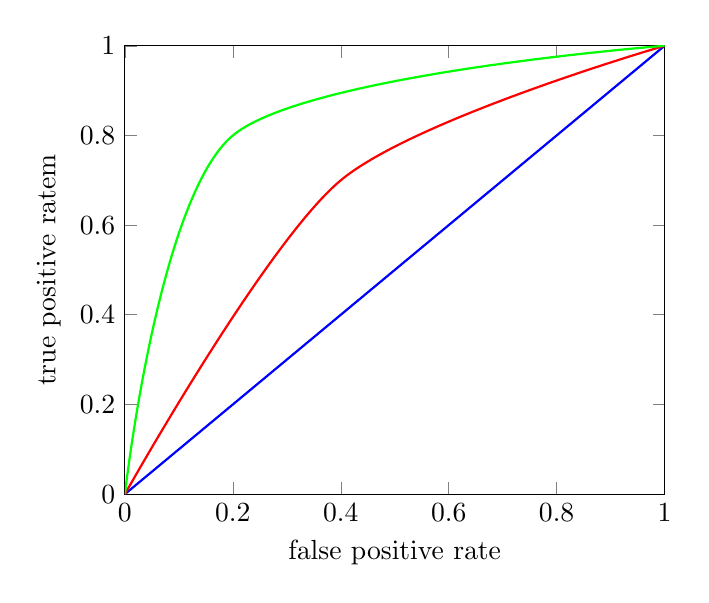
\begin{tikzpicture}
      \begin{axis}[
      	xlabel={false positive rate},
      	ylabel={true positive ratem},
      	ymin = 0, ymax=1, xmin=0, xmax=1,
      ]
      \addplot[thick,smooth,blue]{x};
      \addplot[thick,smooth,red] plot coordinates {
              (0,0)
              (0.4,0.7)
              (1,1)
          };
      \addplot[thick,smooth,green] plot coordinates {
                    (0,0)
                    (0.2,0.8)
                    (1,1)
                };
      \end{axis}
    \end{tikzpicture}
    \caption{ROC curves}
\end{figure}

\subparagraph{Limitations}
\label{subp:limitations}
As mentioned by Powers et al.~\cite{powers2007}, recall, precision, F-measure have a bias.
Recall, precision and F-measure ignore performance in correctly handling negative examples, they propagate the marginal Prevalences and biases, and they fail to take account the chance level performance.
Another drawback or limitation with the measuring of user predictions is that it does not take into account the ranking of the items. To handle this, rank based metrics can be used.

\paragraph{Rank Based Metrics}
\label{para:rank_based}
Rank accuracy metrics measure the ability of a recommendation method to produce
a recommended ordering of items that matches how the user would have ordered
the same items. Shani et al.~\cite{Shani2011} lists two different approaches
for measuring the ranking accuracy: Try determining the correct order of a set
of items for each user and measure how close a system comes to this correct
order, or we can attempt to measure the utility of the system's ranking to a
user.

Herlocker et al.~\cite{Herlocker2004} argue that rank accuracy metrics may be
overly sensitive for domains where the user just wants an item that is `good
enough' (binary preferences) since the user won't be concerned about the
ordering of items beyond the binary classification. These metrics are therefore
most suitable to evaluate algorithms that are used to present ranked lists to
the user in domains where the user preferences are expressed using numerical
values.

\subparagraph{AP correlation}
\label{subp:ap_correlation}
$AP correlation$~\cite{Yilmaz:2008:NRC:1390334.1390435} measures the overall precision and is a variant of $Kendall's$ $tau$.
It counts the amount of items correctly placed in a ordered predicted rank list $list1$ and a list of the actual rank ordering of the preferences of the user $list2$.
\begin{equation}
	AP = \frac{2}{N - 1} * \sum_{i=2}^{N}{(\frac{C(i)}{i - 1})} - 1
	\label{equation:ap}
\end{equation}
How to calculate the $AP correlation$ value is shown in ~\ref{equation:ap}.
$C(i)$ is the number of items ranked correctly above rank $i$.
The value of AP is between -1 and 1, where a score of 0 means that $list1$ can be considered a randomly generated list and 1 is a perfect match with the actual list $list2$.
% \paragraph{Limitations}
% todo maybe

\label{par:accuracy_ranking}

\marginpar{if this is the setup, write a little intro}

\subparagraph{Mean Percentage Ranking (MPR)}
\label{subp:mean_percentage_ranking_}
This measure is a recall-oriented metric.
A known issue with implicit feedback is that it often lack the actual user's preference.
This approach is used to measure the user satisfaction of items in an recommended ordered list.
\begin{equation}
	MPR = \frac{\sum_{u,i}{r_{ui} * rank_{ui}}}{\sum_{u,i}{r_{ui}}}
	\label{equation:mpr}
\end{equation}
How to calculate $MPR$ is shown in~\ref{equation:mpr}.
A list of all the items for user $u$ is ordered based on the rank $rank_{ui}$ of the $u$.
Where $rank_{ui}$ is the percentile rank of item $i$ in this list for $u$.
$rank_{ui} = 0$ means that $i$ is the most preferred item for $u$.
$r_{ui}$ indicates whether $u$ has consumed $i$ or not.
This makes a $MPR$ value of 0\% to be the most preferred value, and a value of 50\% meaning a near randomly produced list.

\subparagraph{Mean Average Precision (MAP)}

\label{subp:mean_average_precision_map_}
MAP~\cite{Manning:2008:IIR:1394399} measures quality across recall levels.

\begin{equation}
	ap@n = \sum_{k=1}^{n}{\frac{P(K)}{min(m,n)}}
	\label{equation:apn}
\end{equation}
\begin{equation}
	MAP@n = \sum_{i=1}^{N}{\frac{ap@n_i}{N}}
	\label{equation:map}
\end{equation}

How to calculate the $MAP$ value is shown in~\ref{equation:map}.
\ref{equation:apn} calculates the average precision at $n$ for a user.
From \ref{equation:apn}, $P(K)$ is the precision at $k$ in the item list, $n$ is the maximum number of predicted items and $m$ is the actual length of the predicted items list.
\ref{equation:map} calculates the mean of all the values from \ref{equation:apn}.

\subparagraph{Normalized Discounted Cumulative Gain (nDCG)}
\label{subp:normalized_discounted_cumulative_gain_}

$nDCG$ measures the graded relevance of the recommended item, the ranking quality or the usefulness of the recommended item based on its rank position.
It is often used to measure the performance of web search recommendation systems.

\begin{equation}
    DCG_k = \sum_{i=1}^{k}{\frac{2^{rel_i}-1}{log_2(i+1)}}
    \label{equation:dcg}
\end{equation}

\begin{equation}
    nDCG_k = \frac{DCG_k}{IDCG_k}
    \label{equation:ndcg}
\end{equation}

How to calculate the $nDCG$ value is shown in~\ref{equation:ndcg}.
Where $k$ is the maximum amount of suggested items, and $rel_i$ is the graded relevance of the result at position $i$.
$IDCG_k$, from~\ref{equation:ndcg}, is the ideal $DCG_k$ value.
This is the result list sorted on relevance.

\subparagraph{Half-life utility~\cite{Breese:1998:EAP:2074094.2074100}}

Assume that the further down an item is in the list the less chance there is for that item to be viewed by the user.
The rate of the decaying probability is exponential.

\begin{equation}
	HL_u = \sum_{i}{\frac{\delta(i)}{2^{\frac{i-1}{\alpha-1}}}}
\end{equation}

$\delta(i)$ is 1 if the user is interested in the item at position $i$ and 0 if not.
$\alpha$ is the viewing half-life, or half-life parameter.
The half-life utility of all the users are shown in~\ref{equation:HL}

\begin{equation}
	HL = 100 * \frac{\sum_u{HL_u}}{\sum_u{HL_u^{max}}}
	\label{equation:HL}
\end{equation}

$HL_u^{max}$ is the maximum possible value of the half-life utility value.
% \paragraph{Limitations}
% todo maybe
\marginpar{some overlapping of the algorithms (not really comparing two ranked list, but still evaluating a recommender system producing ranked lists)}

\marginpar{something like this perhaps}
% paragraph accuracy_ranking (end)


\paragraph{Beyond Accuracy}
There is an emerging understanding that good recommendations accuracy alone does not give the users of the recommender system an effective and satisfying experience \cite{Herlocker2004}. The following \emph{measures} attempts to assess a recommender systems usefulness beyond being able to provide accurate recommendations to the users.

\subparagraph{Coverage}
The term coverage can refer to several distinct properties of the system. Most
commonly, the term coverage refers to the proportion of items the
recommendation system can recommend, also known as \emph{item-space coverage}.
The simplest measure of catalog coverage is the percentage of all items that
can ever be recommended. Coverage can also be the proportion of users
interactions for which the system can recommend items, known as
\emph{user-space coverage}. In many applications the recommender system may not
provide recommendations for some users due to e.g.\\ low confidence in the
accuracy of predictions for that user. In such cases one may prefer a
recommender that can provide recommendations to a wider range of users. However, an increase in coverage is only beneficial if the accuracy does not drop significantly.

\subparagraph{Perceived quality}
To gather the perceived quality the system must ask the user to examine the recommended item, and give feedback regarding the their actual interest in the recommended item.
For the feedback from the user to be as complete as possible, the system must supply the user with the reason to why the item was suggested, and the metadata of the item.
When the user has this overview of the item, the user's feedback regarding the item can produce some quality measure.
One  way of having the user to give this feedback is to re-rate the recommended item on a similar scale as the item was rated.
A rating scale from 1 to 5 is often used for both~\cite{Schafer:1999:RSE:336992.337035}.

\subparagraph{Novelty and Serendipity}
Some recommender systems produce highly accurate recommendations and also have reasonable coverage - and yet that are useless for practical purposes. For instance, a music recommender can recommend Rihanna to every customer who have not yet listened to Rihanna. However, statistically, this is highly accurate as most people have listened to Rihanna or at least knows about her and have consciously chosen not to listen to her. Much more valuable would be a recommendation to a kick-ass indie-rock band that the active user would love, but will never hear about in the news. We therefore need a new dimension for analyzing recommender systems that consider "nonobviousness" of the recommendations. One such dimension is \emph{novelty}. Another related dimension is \emph{serendipity}. A serendipitous recommendation helps a user find a surprisingly interesting item the user might not have discovered otherwise. To clarify the difference between the two, a novel recommendation could be to recommend an unknown album from one of the users favorite artists, that the user likely eventually would have discovered herself. However, a recommendation by an unknown artist is more likely to be serendipitous. Serendipity is therefore a measure of how surprisingly the successful recommendations are.

As novelty is the the degree of new and interesting items recommended for the user, the system must ask the user for feedback to be able to make any assumptions around the novelty.
The novelty together with perceived quality allows the system to make informed decisions about the ratio of new items to recommend for the user.
The novelty is expected to change over time, some times the user would like to receive recommendation on new items, and other times recommendations closer to the user's preferences.
For the system to be able to detect these changes in preferences, and acting accordingly would be beneficial in regards of the user's satisfaction.
\begin{equation}
    Novelty(u) = \frac{1}{N}\sum_{i=1}^{N}{1 - Knows(u,i)}
    \label{equation:novelty}
\end{equation}
In~\ref{equation:novelty} $Knows(u,i)$ represents a binary functions which returns 1 if the user $u$ knows the item $i$, and 0 if not.
The set of items used for the calculation is the set of recommended items for the user.

The system should be able to produce items both items known to the user, and items unknown to the user.
For trust in the system and novelty respectively.

\begin{figure}[H]
    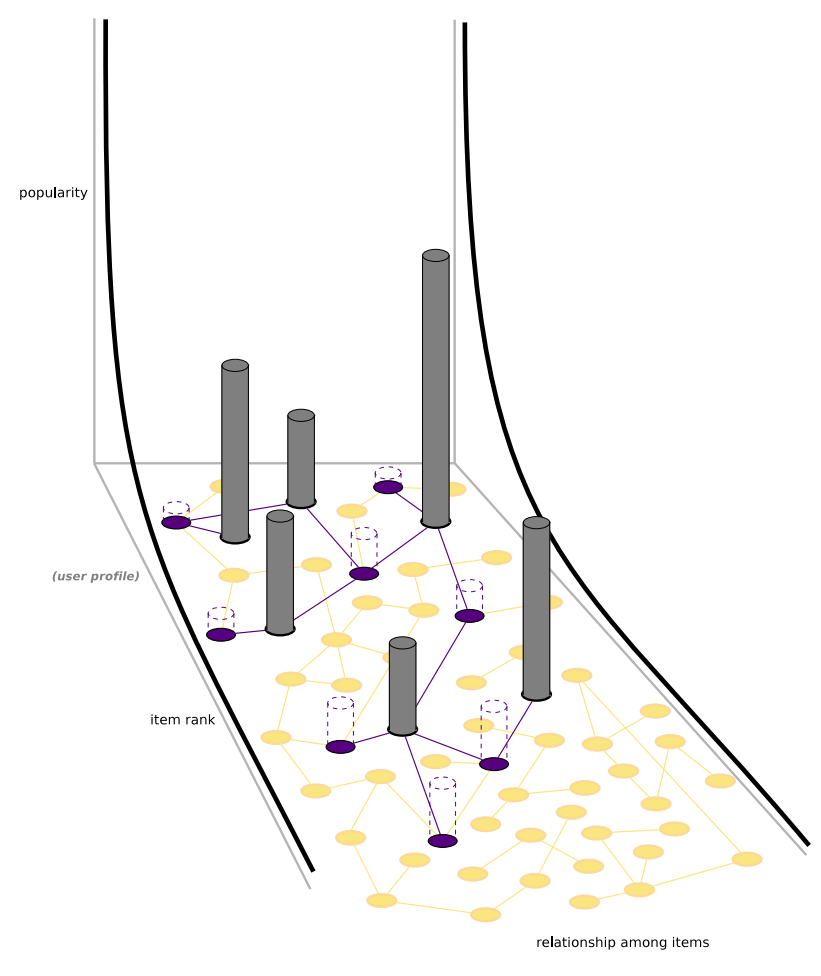
\includegraphics[width=5in]{image/longtailNoveltyFig.png}
    \centering
    \caption[Long tail]{Long tail show with the item similarity between items. Similarity shown though edges between the nodes. The gray columns represents the user profile, the violet represents items which might be of interest to the user, and the height is the relevance. Adapted from~\cite{celma2008}}
    \label{figure:longtailNovelty}
\end{figure}
\marginpar{todo - not sure if its ok to use this image (not self made) figure from music recommendation, but long tail applies to fashion}
\marginpar{todo - if so, something about longtail}

\subparagraph{Diversity}
Diversity is generally defined as the opposite of similarity. In some cases suggesting a set of similar items may not be as useful for the user, because it may take longer to explore the range of products. E.g. when presenting a list of 5 recommendations, the system should not recommend 5 Ralph Lauren shirts with different colors. As diversity may come at the expense of other properties such as accuracy, one should evaluate the decrease in accuracy vs. the increase in diversity.

Other evaluation methods worth knowing about includes confidence, trust, utility, robustness, adaptivity, scalability mentioned in \cite{Herlocker2004, Shani2011}.

\subparagraph{User-Centric Evaluation}
User-centric evaluation focuses on the perceived quality of the recommendation system~\cite{Pu:2011:UEF:2043932.2043962,Knijnenburg:2011:PPS:2043932.2043993}.
To gather this kind of information, user feedback is required.
User-centric evaluation is meant to handle the short comings of the offline evaluation metrics, such as predictive accuracy metrics.
User-centric evaluation can make evaluations on items which the user has not yet show interest in.
This allows user-centric evaluation to make evaluations on information about the system, such as the perceived quality and novelty of the recommendation system.
When the user feedback has been gathered the data must be analyzed.

\marginpar{move offline beyond accuracy to here maybe? }


\subsubsection{Evaluation using Implicit Feedback}
Accuracy metrics such as RMSE and MAE are not especially well suited for implicit feedback datasets, as they require knowing which items are undesired by a user~\cite{Hu2008}.
One way to handle the issue with missing negative feedback is through conversion of the implicit feedback to explicit feedback, and thereby producing a sense of negative feedback.
One issue with this is what is considered as negative feedback in the sense of implicit feedback.
The reason for a user not to access an item is not necessarily grounded in dislike, but could simply be an overlook.
On the other hand, if the user accessed the item for a short time without buying it, the user might not like it.
These questions raises the need for a different approach when wanting to measure a recommender system using implicit feedback.

Joachims et al.~\cite{Joachims07evaluatingthe} shows that clicks can be biased, and has to be interpreted relative to the order of presentation and relative to the other abstracts.

\marginpar{extend}

Two ways of measuring the system is through ranking and usage prediction described earlier.

\paragraph{Rank Based} % (fold)
	\label{par:Ranking_based}
	The ranking approach can be considered more suited to test recommendation systems using implicit feedback since a subset of the items are meant to be recommended to the user.
	This subset is usually a ranked top K list of items where the items in this list is the items the system predicts will be most liked by the user.

	One issue with this approach is that the items in the predicted top K list has to be ranked in some way, the same goes for the list this list is to be compared to.
	Thereby producing the requirement for a ranked list of preferred items from the user.
	If there is such a ranked list, ranking accuracy will help to tell how well the system is suggesting items for the user, such as~\cite{Yilmaz:2008:NRC:1390334.1390435}.
% paragraph paragraph_name (end)

\marginpar{maybe hard to differentiate between the names}

\paragraph{Accuracy Ranking} % (fold)
	\marginpar{HELGE: Språk!}
	\label{par:usage_prediction}
	When there is lack of explicit user feedback and a ranked list of the items cannot be produced, ranking the predicted list and scoring this list based on the actual user preferences can be used to evaluate the system.
	The actual user preferences are a list of binary preferences for the items.
	This list is often possible to construct from implicit feedback, but will seldom be a complete list, and most often be a list with only positives (not possible to produce not interesting).
	Some of the different approaches when dealing with implicit feedback are:
	Li et al.~\cite{deLace2010} who used $MPR$ and $MAP$ to calculate their performance.
	Pan et al.~\cite{Pan:2013:GGP:2540128.2540516} who used a set of top-k evaluation metrics: precision, recall, F1, nDCG, ROC and 1-call.
	Sindhwani et al.~\cite{Sindhwani:2010:OMC:1933307.1934641} who used roc curve and precision-recall curve to evaluate their experiments.
	Pan et al.~\cite{pan2008} who used $MAP$ and Half-life Utility.

	$nDCG$, $MAP$ and Half-life utility has a similar setup.
	They all have a decaying factor, and rewards the system in different ways for how high in the list a relevant recommended item is.

	On the other hand metrics as Precision alone has no decaying factor, and will not penalize a system with uninteresting items suggested higher in a ranked list.

	% \cite{Nati03weightedlow-rank} average squared difference
% paragraph usage_prediction (end)

	%TODO - What evaluation measures are suited for implicit feedback, and why are traditional evaluation measures such as RMSE, ... not as suitable when working with implicit feedback?

\subsubsection{Evaluation of Cold-start Recommendations}
\label{sec:cold-start-eval}
\marginpar{Helge: Pros og Cons plz}
\marginpar{Fix pros pg cons, for mye "synsing}

The cold-start problem can be considered a sub problem of coverage. The cold-start
problem occurs when the recommender system cannot draw any inferences for user or items
which it has not yet gathered sufficient information. When
evaluating the cold-start system performance one is interested in measuring the
system accuracy for these users and items.

The evaluation metric used depends on the type of feedback available.
Most experiments carried out have used \emph{traditional} explicit feedback datasets such as
MovieLens, EachMovie, Netflix etc. Accuracy metrics such as MAE~\cite{Rashid2002, Rashid2008, Massa2004,
Massa2007, Stern2009} and RMSE~\cite{Agarwal2009, Agarwal2010} are therefore
the most used ones. In the experiments where binary rating data have been used
Precision@N~\cite{Liu2011, Gantner2010}, ROC curves~\cite{Agarwal2009,
Gantner2010, Schein2002} and Area Under Curve (AUC) \cite{Liu2011, Gantner2010} seems to be the
preferred evaluation metrics.

Another way to discriminate between different recommender techniques is
coverage. The recommender system may not be able to make predictions for every
item. For this reason, it is important to measure the portion of ratings that
an RS is able to predict (ratings coverage). However, this quantity is not
always informative about the quality of a recommender system. A RS is likely to
be good at predicting nearly all the ratings for heavy users and not be able to
do the same for users who have rated few items. For this reason, one should
also compute the users coverage, defined as the portion of users which the RS
is able to predict at least one rating for. Good et al.~\cite{Good1999}
measure the item-space coverage, while Massa et al.~\cite{Massa2004,
Massa2007} measures both the item-space coverage and user-space coverage of
their methods.

Massa et.\ al~\cite{Massa2004} argue that performance measures such as Mean
Absolute User Error (MAUE) is a good measure for cold-start recommendations
since every user is taken into account once and a cold start user is as
influential as an heavy rater. Similarly, Park et al.~\cite{Park2006} measure
normalized MAE (NMAE) by macro-averaging, which first calculates the mean
average error of each users and taking the average of all users.

To simulate the cold-start scenario, different approaches have been employed:
One popular way to simulate a cold-start user scenario used by~\cite{Stern2009,
Lam2008} is to split the dataset in two disjoint sets, a training set
containing 90\% of the users and the remaining 10\% being in the test set. For
each test user one trains a model with a random subset $T\%$ of their ratings
e.g.\ $5\%$ or $75\%$, and then use the model to predict their remaining
ratings. The same methodology can also be used to simulate a cold-start item
scenario. Another highly similar way to simulate the cold-start user and
cold-start item scenario was used in~\cite{Rashid2002, Rashid2008}. For the
cold-start user scenario one selects a subset of the users with e.g.\ more than
200 ratings. One then trains the model with a subset of the ratings. In the
case of~\cite{Rashid2002} 30, 45, 60 and 90 ratings was used. After training
the model one computes the error on the hidden ratings for the same user.
Stern et. al. \cite{Stern1998} also used a similar method which they called Given $n$, in which
they trained their model using 2, 5 and 10 ratings for each test user and predict
the remaining values.

%Pros & Cons
The advantage of the latter approach is that they use a selection criteria for the test users
to avoid users with really few ratings which might be crucial on a cold-start dataset.
The obvious problem with this approach is that for cold-start datasets these users might stand for a large portion of the ratings. There are both pros and cons of using a fixed subset of ratings rather than using the percentage of ratings, the best choice will most likely depend on the dataset. Using a fixed subset of ratings would be preferable e.g. if the number number of ratings given by the users are fairly uniform.

Another \emph{simpler} approach employed by~\cite{Massa2007, Jamali2009} is to
determine a cutoff point for what is considered a cold-start user. E.g.\ that
every user with less than 5 ratings is considered a cold-start user. Then
separately measure the error on predictions made to these users.

%Pros & Cons
The problem with this approach is that it does not measure how well the recommendation quality improves as
users provide an increasing amount of ratings, giving a less detailed view of the systems performance.
The number of ratings predicted is also likely to be fairly small given a cold-start dataset.

To simulate a cold-start system scenario Agarwal et al.~\cite{Agarwal2009}
split the dataset in two using 75\% of the dataset for training and 25\% for
testing. They then train the model using 30\%, 60\% and 75\% of the data and
compare their performance on the testset.

%Pros & Cons
Good and simple model as it is likely to generate three different training sets
with different sparsity levels, which is exactly what we want to test. However,
if the training examples are drawn at random the experiment should be repeated multiple
times to avoid getting \emph{unfortunate} splits.


%Summary of articles read

%	What evaluation metrics are used?

%\cite{Rashid2008}: Accuracy metric: MAE, Expected Utility (Penalize false positives more than false negatives)
%\cite{Rashid2002}: Accuracy metric: MAE
%\cite{Massa2004}: Leave one out, MAE, MAUE, Rating Coverage, User Coverage
%\cite{Massa2007}: Leave one out, MAE, MAUE, Rating Coverage, User Coverage,
%\cite{Jamali2009}: Leave one out, Recall/Hit-ratio
%\cite{Agarwal2009}: Movie: RMSE, Yahoo: ROC curves, 5-fold cross validation
%\cite{Agarwal2010}: RMSE, True Positive Rate, True Positive Rate
%\cite{Liu2011}: Precision at N, Mean average precision, area under curve
%\cite{Park2006}: NMAE
%\cite{Good1999}: Coverage, MAE, ROC
%\cite{Stern2009}: MAE
%\cite{Ganter2010}: Precision at N (5 & 10), AUC (General ranking measure)
%\cite{Schein2002}: GROC (hit/miss rate)

%	What type of user feedback is used?

%\cite{Rashid2008}: Explicit feedback, MOVIELENS, Only users with 80 or more ratings
%\cite{Rashid2002}: Explicit feedback, MOVIELENS, Only users with 200 or more ratings
%\cite{Massa2004}: Explicit feedback, EPINIONS + Web of trust
%\cite{Massa2007}: Explicit feedback, EPINIONS + Web of trust
%\cite{Jamali2009}: Explicit feedback, EPINIONS + Web of trust
%\cite{Agarwal2009}: Explicit feedback, MovieLens + EachMovie, also incorporates user features
%\cite{Agarwal2010}: Explicit feedback + User features and bag of words rep of crawled movie data - MovieLens, Yahoo! Buzz (1 or -1), BookCrossing
%\cite{Liu2011}: Explicit feedback. Netflix...
%\cite{Park2006}: Explicit feedback, Yahoo!, MovieLens, EachMovie
%\cite{Stern2009}: MovieLens, Netflix,
%\cite{Ganter2010}: MovieLens - Binary (likes, not likes)
%\cite{Schein2002}: MovieLens, Movielens(Stripped of ratings -> implicit)

%	How do they similate the "cold-start situation"?

%\cite{Rashid2008}: Use the movies found when presenting 15, 30, 45, 60, 75 movies to provide predictions for the remaining movies in the list of each user
%\cite{Rashid2002}: Use the movies found when presenting 30, 45, 60, 90 movies to provide predictions for the remaining movies in the list of each user
%\cite{Massa2004}: Consider users who provided 2, 3 or 4 ratings, How does trust propagation of 1,2,3,4 affect rating & user coverage and predictive accurracy?
%\cite{Massa2007}: All users, cold users, heavy users, Controversial items, Black sheep, Trust propagation performance on entire dataset
%\cite{Jamali2009}: All users, cold start users (<5 ratings), recall for different neighborhood sizes
%\cite{Agarwal2009}: 25\% set aside for evaluation, train each model with 30\%, 60\%, 75\% of data, compare performance
%\cite{Agarwal2010}:
%\cite{Liu2011}: User cold start: Split users into disjoint sets (training, test). Item cold start: Split into disjoint sets
%\cite{Park2006}: Fraction of training data used [0.1 -> 1.0]. Cold-start user: Select users with more than 40 ratings in the training set and more than 1 in the test set. Split into 5, with 20\% of the users in each training set. Starting at 2 ratings, add 2 additional training set ratings per iteration until 40 ratings are added. Take the average of the 5 to compute the NMAE. Cold-start item: Items rated by more than 40 users in training data, and at least 1 user in test set. Split in 5. Starting from 2, add 2 more users per iteration. Take average NMAE from each split.
%\cite{Stern2009, Lam2008}: Divide users in two sets (90:10), train model on the 90\%. For each test user train the model on a random subset of T\% of their ratings for T = 5, T=75, then use the model to predict the remaining ratings for the user

%Clues
% http://delivery.acm.org/10.1145/570000/564421/p253-schein.pdf?ip=129.241.103.83&id=564421&acc=ACTIVE%20SERVICE&key=CDADA77FFDD8BE08%2E5386D6A7D247483C%2E4D4702B0C3E38B35%2E4D4702B0C3E38B35&CFID=419807217&CFTOKEN=62708098&__acm__=1394537427_86c608d0d7733db023faa5a09da46de7

\subsection{Online Evaluation}

Instead of doing offline evaluations on the system, one could also run large
scale experiments on a deployed system. Such experiments evaluate the
performance of recommender systems on real users which are oblivious to the
conducted experiment. The real effect of a recommender system depends on a
variety of factors such as user’s intent, the user’s context and how the
recommendations are presented to the user. All these factors are hard to
capture in an offline setting. Thus, the experiment that provides the strongest
evidence as to the true real value of the system is an online evaluation, where
the system is used by real users to perform real tasks.

\subsubsection{Online Evaluation Metrics}

Online studies in recommendations and advertisement usually measure the
click-through-rate (CTR) of the recommendations, which aligns with financial
incentives and implicitly factors in accuracy, novelty, diversity, etc.,
according to the preferences of the distribution of users.  The
click-through-rate of an algorithm is defined as the number of clicks your
recommendations get divided by the total number of recommendations that have
been made. A high CTR therefore indicates that your system is doing well.

\begin{equation}
CTR = \frac{Clicks}{Recommendations}
\end{equation}

\subsubsection{A/B Testing}
	A/B testing or bucket testing is used to test a system on live audience.
	In its' simplest form the audience is split into two groups, but it is also possible to make multiple groups of users.
	The different groups are presented with different altered versions of the system and is asked to use the system as they normally would.
	The goal is to figure out which version is producing the best results, whether it is user satisfaction or revenue.
	How the altered versions are scored is usually done trough a measure of the applications main goal, for instance with an e-commerce application where the main goal is to sell items, the score could be revenue produced by that version.

\paragraph{Example}
	In the case with the SoBazaar application, on way of doing a A/B testing on the system is as follows:
	3 groups of users are made, one with the unaltered system, one with method $A$ to produce recommendations and one with method $B$.

\subparagraph{Group Split} % (fold)
\label{par:group_split}
	The groups of users can either be selected to fit the global distribution of users, or be a set of similar minded users.
	The latter case might benefit a system where the intended goal is to specialize the system for a set of users, or actually partition the system into fitting a subsets of its' users.

\subparagraph{Group Size} % (fold)
  \label{par:group_size}
	The size of the groups depends on the amount of splits and intended stability of the system.
	The group with the original system will be the biggest group to maintain the established image of the application.
	For a system with a well established image, and a large set of faithful users, changes in the system might produce unwanted results.
	The two groups with the altered versions of the system can be of the same size to make it simpler to measure the performance of the two system against one another.

\subparagraph{System Measuring} % (fold)
\label{par:system_measuring}
	After a set period of time, the two altered versions are compared to one another and the original system.
	This is done trough measuring either the revenue produced or clicks.
	For a recommender system it is not just interesting to look at the final income number, but also if the user actually showed any interest in the products recommended for the users.
	If a larger portions of the users from version $A$ showed an increased interest in the recommended items compared to the users from version $B$, that might indicate that version $A$ is a stronger system than system $B$

\paragraph{Disadvantages}
	An issue with A/B testing is that when splitting the users into subgroups of users, these subgroups might not possess the same user properties as the complete set of groups had.
	This might lead to a biased score for the group, which might not reflect the actual score of the system when releasing it on the full set of user groups.


\subsubsection{Multi-armed bandit experiments \cite{googlebandit}}
	
	A multi-armed bandit is a type of experiment where:
	
	\begin{itemize}
	\item The goal is to find the best or most profitable action
	\item The randomization distribution can be updated as the experiment progresses
	\end{itemize}
	
	The "multi-armed bandit" described a hypothetical example where you face several slot machines ("one-armed bandits")
	with potentially different payouts. You wish to find the slot machine with the best payout rate, but you also want to
	maximize your winnings. The fundamental tension is between "exploiting" arms that have performed well in the past
	and "exploring" new or seemingly inferior arms in case they might perform better. 
	
	In normal A/B testing, you will split the traffic equally between both systems, meaning that both get 50\% of the
	traffic each, all the time. When using bandits you can continuously adjust the traffic each variation receives based on its
	performance. Variations that appear to do well gets more traffic, and variations that clearly is underperforming
	gets less. The adjustments are made based on a statistical test that considers both the sample size and performance
	metrics together.
	
	\paragraph{Advantages}
	
	The main advantage of using multi-armed bandit experiments is that it usually performs better than A/B testing
	when we look at average conversion rates, which in turn will decrease the cost of the experiment.
	Saved testing time is another advantage highlighted in the Google article.
		
	\paragraph{Disadvantages}
	
	Statistical significance. Instead of sending equal traffic to each of the test pages, the page which performs
	better will start to get more traffic. If you are running tests across pages which do not get huge amounts of
	traffic, one variant can run away while the others are left in the dust without getting a fair chance. Of course,
	if your variation is performing badly you will loose some sales or conversions in the process of A/B testing,
	but that is the price one have to pay for finding out if a variation really did perform badly.

\subsection{Discussion}
The main idea behind a recommendation system is to produce a set of items which are of interest to the user.
For the system to be successful, this sets of items needs quality.
But what needs to be considered when determining the quality of the recommendations?
According to a user study~\cite{Pu:2011:UEF:2043932.2043962} the most central aspects to this quality is:

% \todo{as list or in table, or not}

\subsubsection{Perceived accuracy}
The degree of how well the user perceives the recommended items match the actual want of the user.

\subsubsection{Novelty}
The degree of new and interesting items recommended for the user.

\subsubsection{Attractiveness}
How well the recommended items are able to evoke interest or desire in the user.

\subsubsection{Diversity}
How different the recommended items are.

\subsubsection{Context compatibility}
How the system uses contextual factors to supply the recommendations with more personalized recommendations.


\subsection{The Good}
Since the data at hand is mainly implicit feedback and this data is sparse, some natural ways of approaching the evaluations task would be:

\subsubsection{MPR}
\begin{itemize}
	\item good
	\item Possible to produce a score for a recommender system which relies on implicit feedback
	\item Usable even though there are no feedback indicating undesired items
	\item Does not need a ranked list of the actual preferences of the user
	\item bad
	\item Needs distinct ranking of the different items
\end{itemize}

\subsubsection{MAP}
\begin{itemize}
	\item good
	\item Possible to produce a score for a recommender system which relies on implicit feedback
	\item Usable even though there are no feedback indicating undesired items
	\item Does not need a ranked list of the actual preferences of the user
	\item Differentiates between predicted more desired items and those that are not
	\item bad
	\item Needs distinct ranking of the different items
\end{itemize}


\subsection{The Bad}
\subsubsection{RMSE}
\begin{itemize}
	\item good
	\item Well known, so it produces a clear score of the system
	\item bad
	\item Needs the actual rating of the items
	\item Needs a predicted rating for the items
	\item Not easy to gather reliable information about undesired items trough implicit feedback
\end{itemize}


